\documentclass[11pt]{beamer}

\mode<presentation>
\usetheme{metropolis}

\usepackage{appendixnumberbeamer}
\usepackage{booktabs}
\usepackage[scale=2]{ccicons}
\usepackage{fontspec}
\usepackage{graphicx}

\usepackage{polyglossia}
\setdefaultlanguage[variant=brazil]{portuguese}

\usepackage{alltt}

\usefonttheme{professionalfonts}
\usepackage{fontspec}
\setsansfont{Fira Sans}
\setmonofont{Fira Mono}

\setbeamertemplate{frame footer}{\href{http://creativecommons.org/licenses/by-sa/4.0/}{\ccbysa}
                                 \footnotesize{ \url{https://github.com/ayharano/just-python/}}}

\graphicspath{ {.} }


\title{\normalsize{Do zero à publicação de um pacote de distribuição no \href{https://pypi.org/}{PyPI}}}
\author{\href{https://alexandre.harano.net.br/}{Alexandre Yukio Harano}}
\institute[.]
{alexandre@harano.net.br\\
 \url{https://alexandre.harano.net.br/}}
\date{\scriptsize{\href{https://justpython.style/}{São Paulo, 14 de Julho de 2018}
 --
\href{https://justpython.style/}{Just Python}}}



\begin{document}

\maketitle

\begin{frame}[standout]
  O que implementar?
\end{frame}

\begin{frame}[fragile]{IPAM - IP Address Management}
  \begin{flushright}
  \begin{itemize}
    \item Gerenciadores de endereços IP: ferramentas em software usadas para planejar, rastrear e gerenciar endereços e subredes.
    \item Usado por administradores de redes corporativas, principalmente Provedores de Serviço Internet (ISPs): administrar redes delegadas, subredes de um bloco IP e endereços de equipamentos.
  \end{itemize}

  \tiny{\vspace*{.25cm}
    Baseado em \url{https://en.wikipedia.org/wiki/IP_address_management}}
  \end{flushright}
\end{frame}

\begin{frame}[fragile]{\href{https://phpipam.net/}{phpIPAM}}
  \hspace*{-.5cm}\centering{\href{https://phpipam.net/}{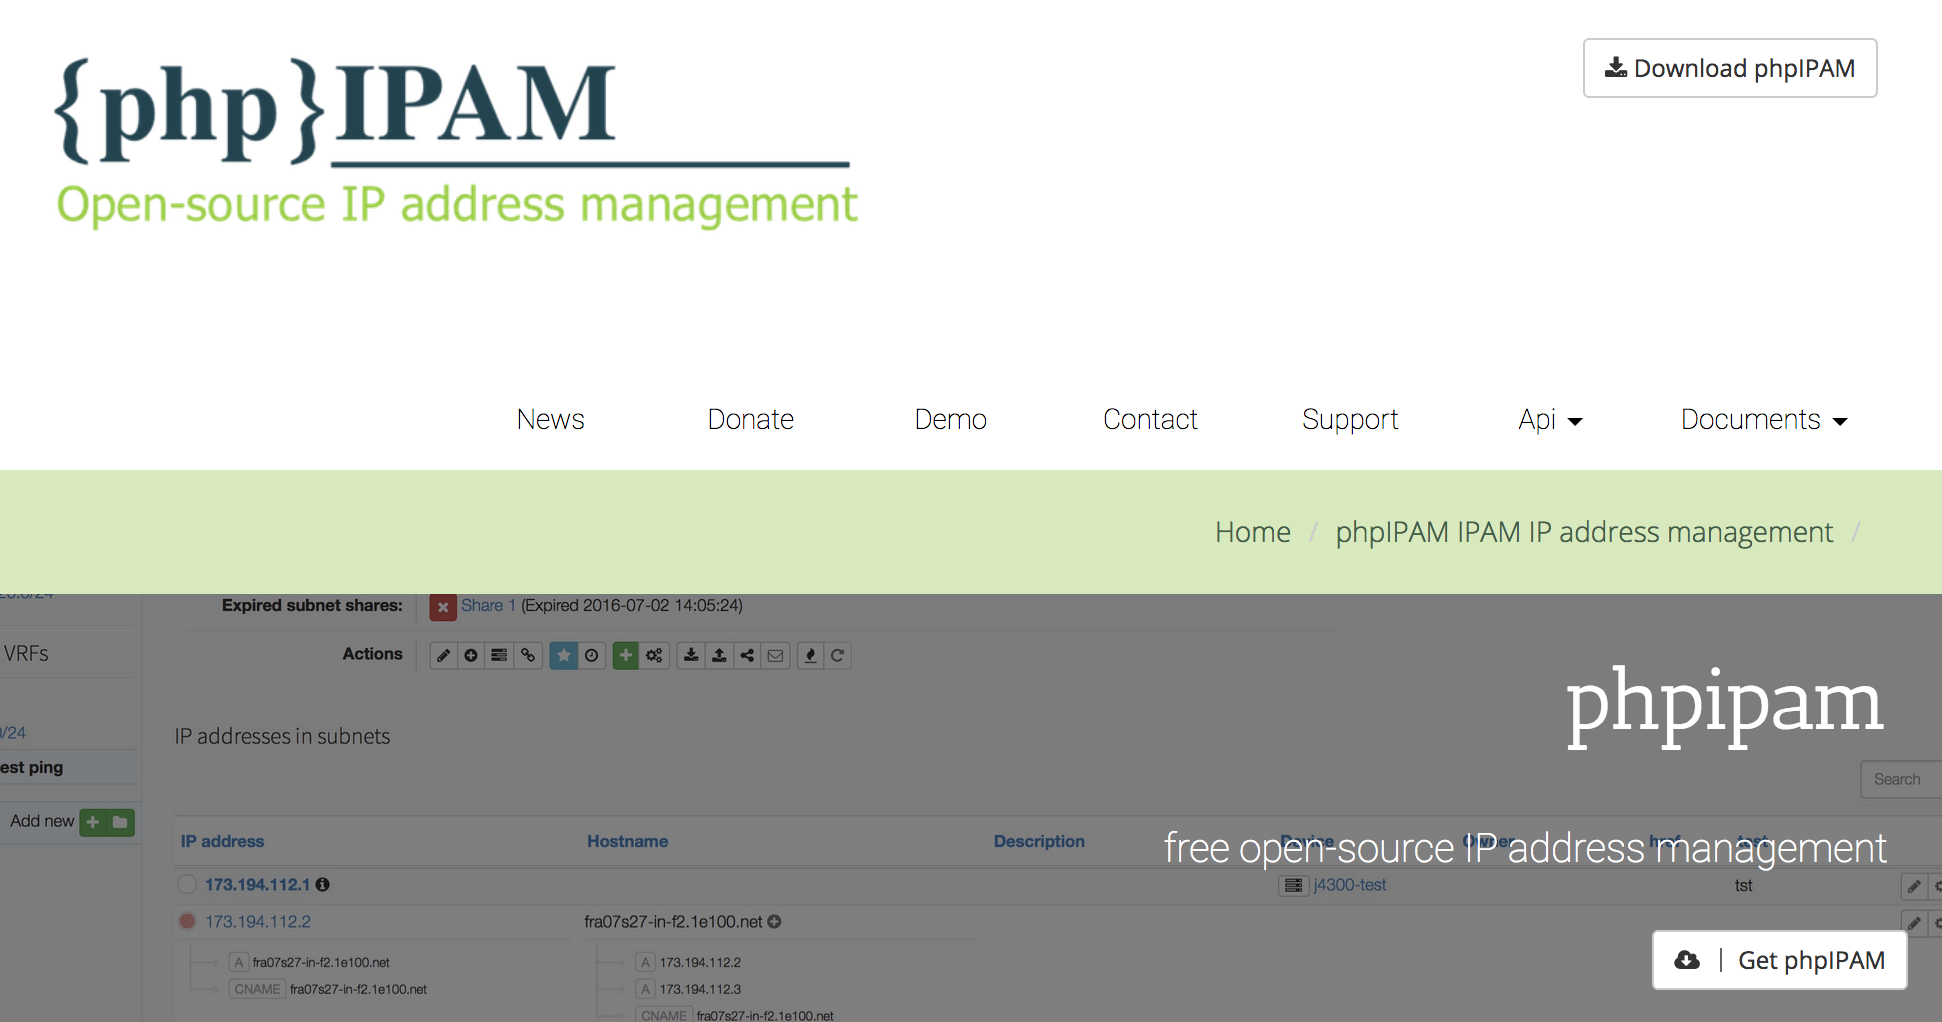
\includegraphics[width=12cm]{phpipam_home}}}
\end{frame}

\begin{frame}[fragile]{\href{https://phpipam.net/documents/features/}{Features do phpIPAM}}
  \hspace*{-.5cm}\centering{\href{https://phpipam.net/documents/features/}{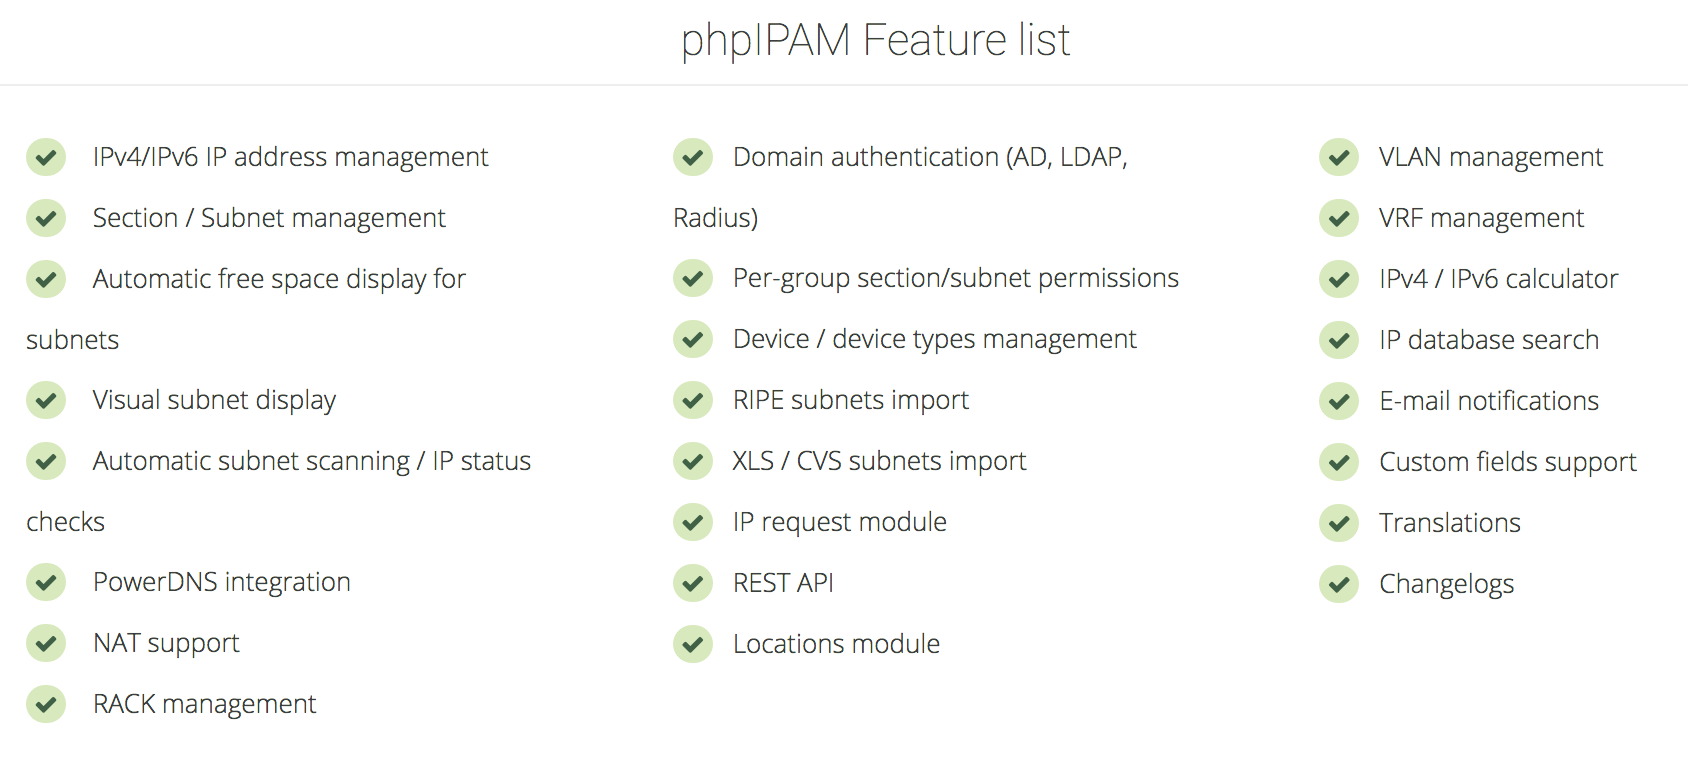
\includegraphics[width=12cm]{phpipam_features}}}
\end{frame}

\begin{frame}[standout]
  E agora?
\end{frame}

\begin{frame}[fragile]{\small{PPPIPAM - Poor's Person Python IP Address Manager}}
  \begin{itemize}
    \item \href{https://www.macmillandictionary.com/dictionary/british/a-poor-man-s-something}{Baseado na expressão \textit{poor's man}: usado para comparar algo menos bem sucedido comparado a outra pessoa: \texttt{He’s a kind of poor man’s James Bond}}.
    \item \textit{Person} em vez de \textit{man} para ser generalista.
    \item Similar ao bem conhecido \href{https://phpipam.net/}{phpIPAM}.
    \item Python no nome.
    \item \href{https://en.wikipedia.org/wiki/Point-to-Point_Protocol_over_Ethernet}{Referência fraca a PPPoE, um protocolo usado em Provedores de Serviço Internet}.
  \end{itemize}
\end{frame}

\begin{frame}[standout]
  Por quê?
\end{frame}

\begin{frame}[fragile]{\href{https://docs.python.org/3/library/ipaddress.html}{\texttt{ipaddress}}}
   \hspace*{-.5cm}\centering{\href{https://docs.python.org/3/library/ipaddress.html}{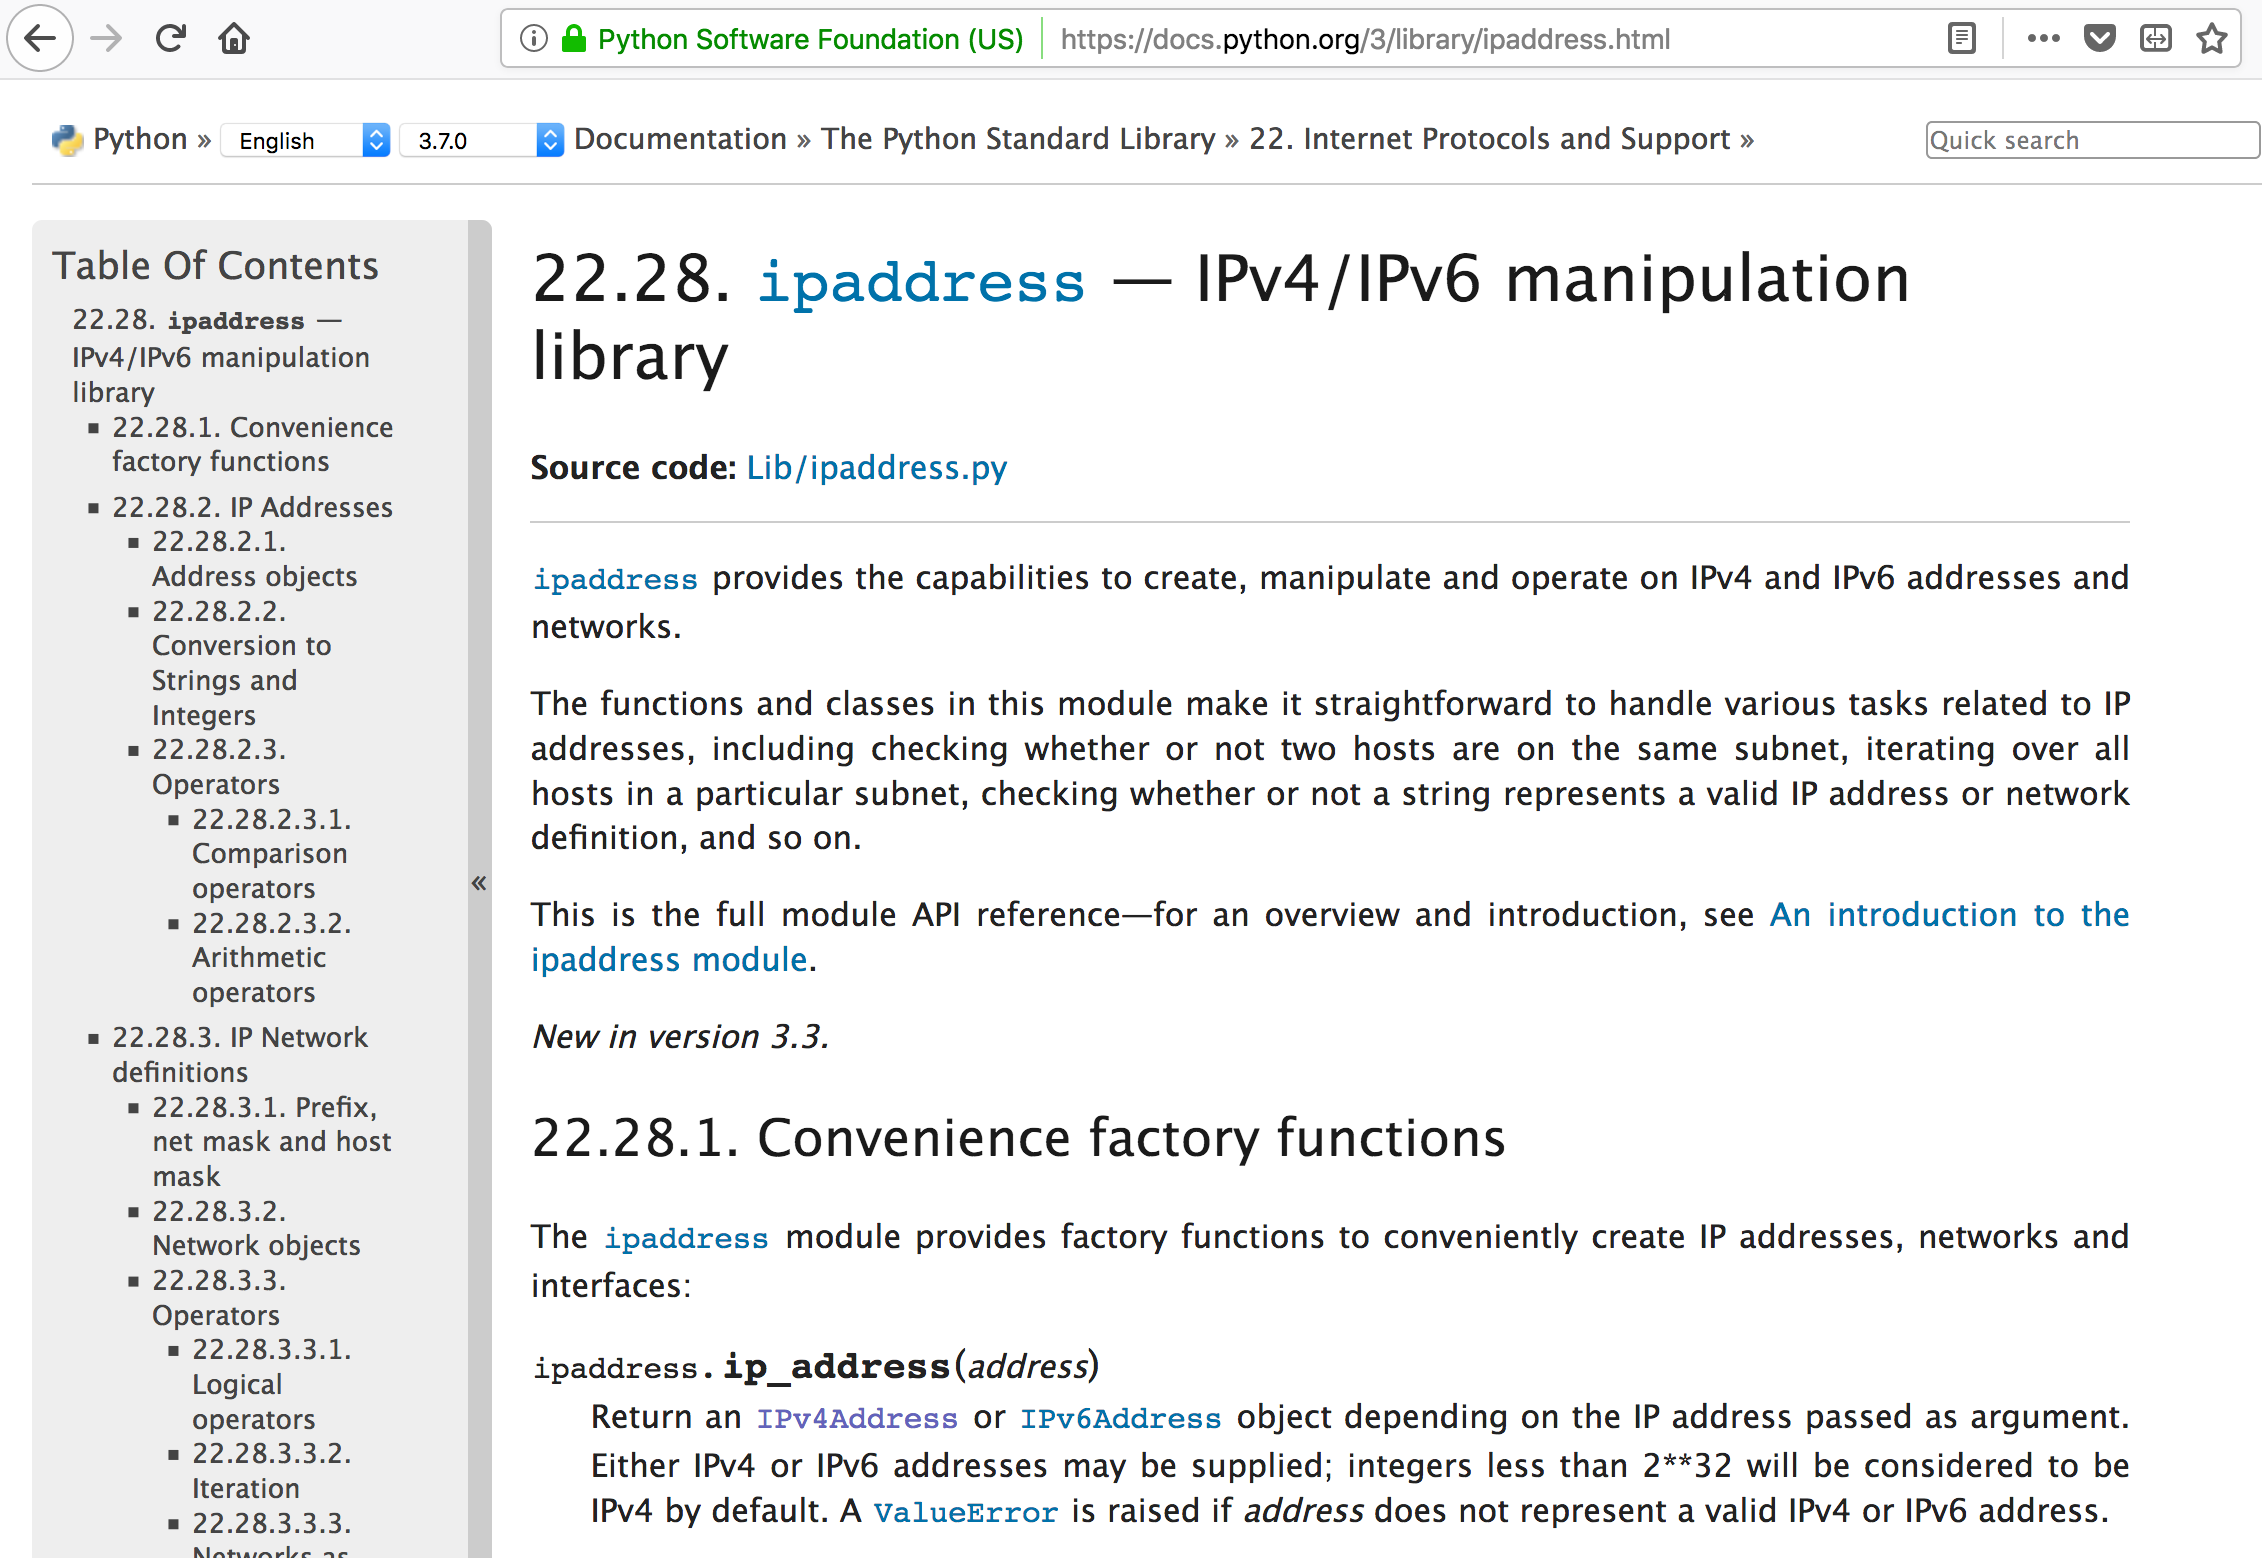
\includegraphics[width=12cm]{ipaddress}}}
\end{frame}

\begin{frame}[fragile]{\href{https://docs.python.org/3/library/ipaddress.html}{\texttt{ipaddress}}}
\hspace*{-2cm}
\vspace*{-1cm}
\begin{alltt}\small
>>> import ipaddress
>>> rede_ipv6 = ipaddress.ip_network(
...     "2001:db8:01a::/64")
>>> endereco_ipv6 = ipaddress.ip_address(
...     "2001:db8:01a::a10")
>>> endereco_ipv6 in rede_ipv6
True
>>> doc_ipv6 = ipaddress.IPv6Network("2001:db8::/32")
>>> doc_ipv6.supernet_of(rede_ipv6)
True
>>> endereco_ipv6.version
6
>>>
\end{alltt}
\end{frame}

\begin{frame}[standout]
  Como começar do zero?
\end{frame}

\begin{frame}[fragile]{\href{https://docs.python.org/3/library/venv.html}{\texttt{venv}}}
  \hspace*{-.5cm}\centering{\href{https://docs.python.org/3/library/venv.html}{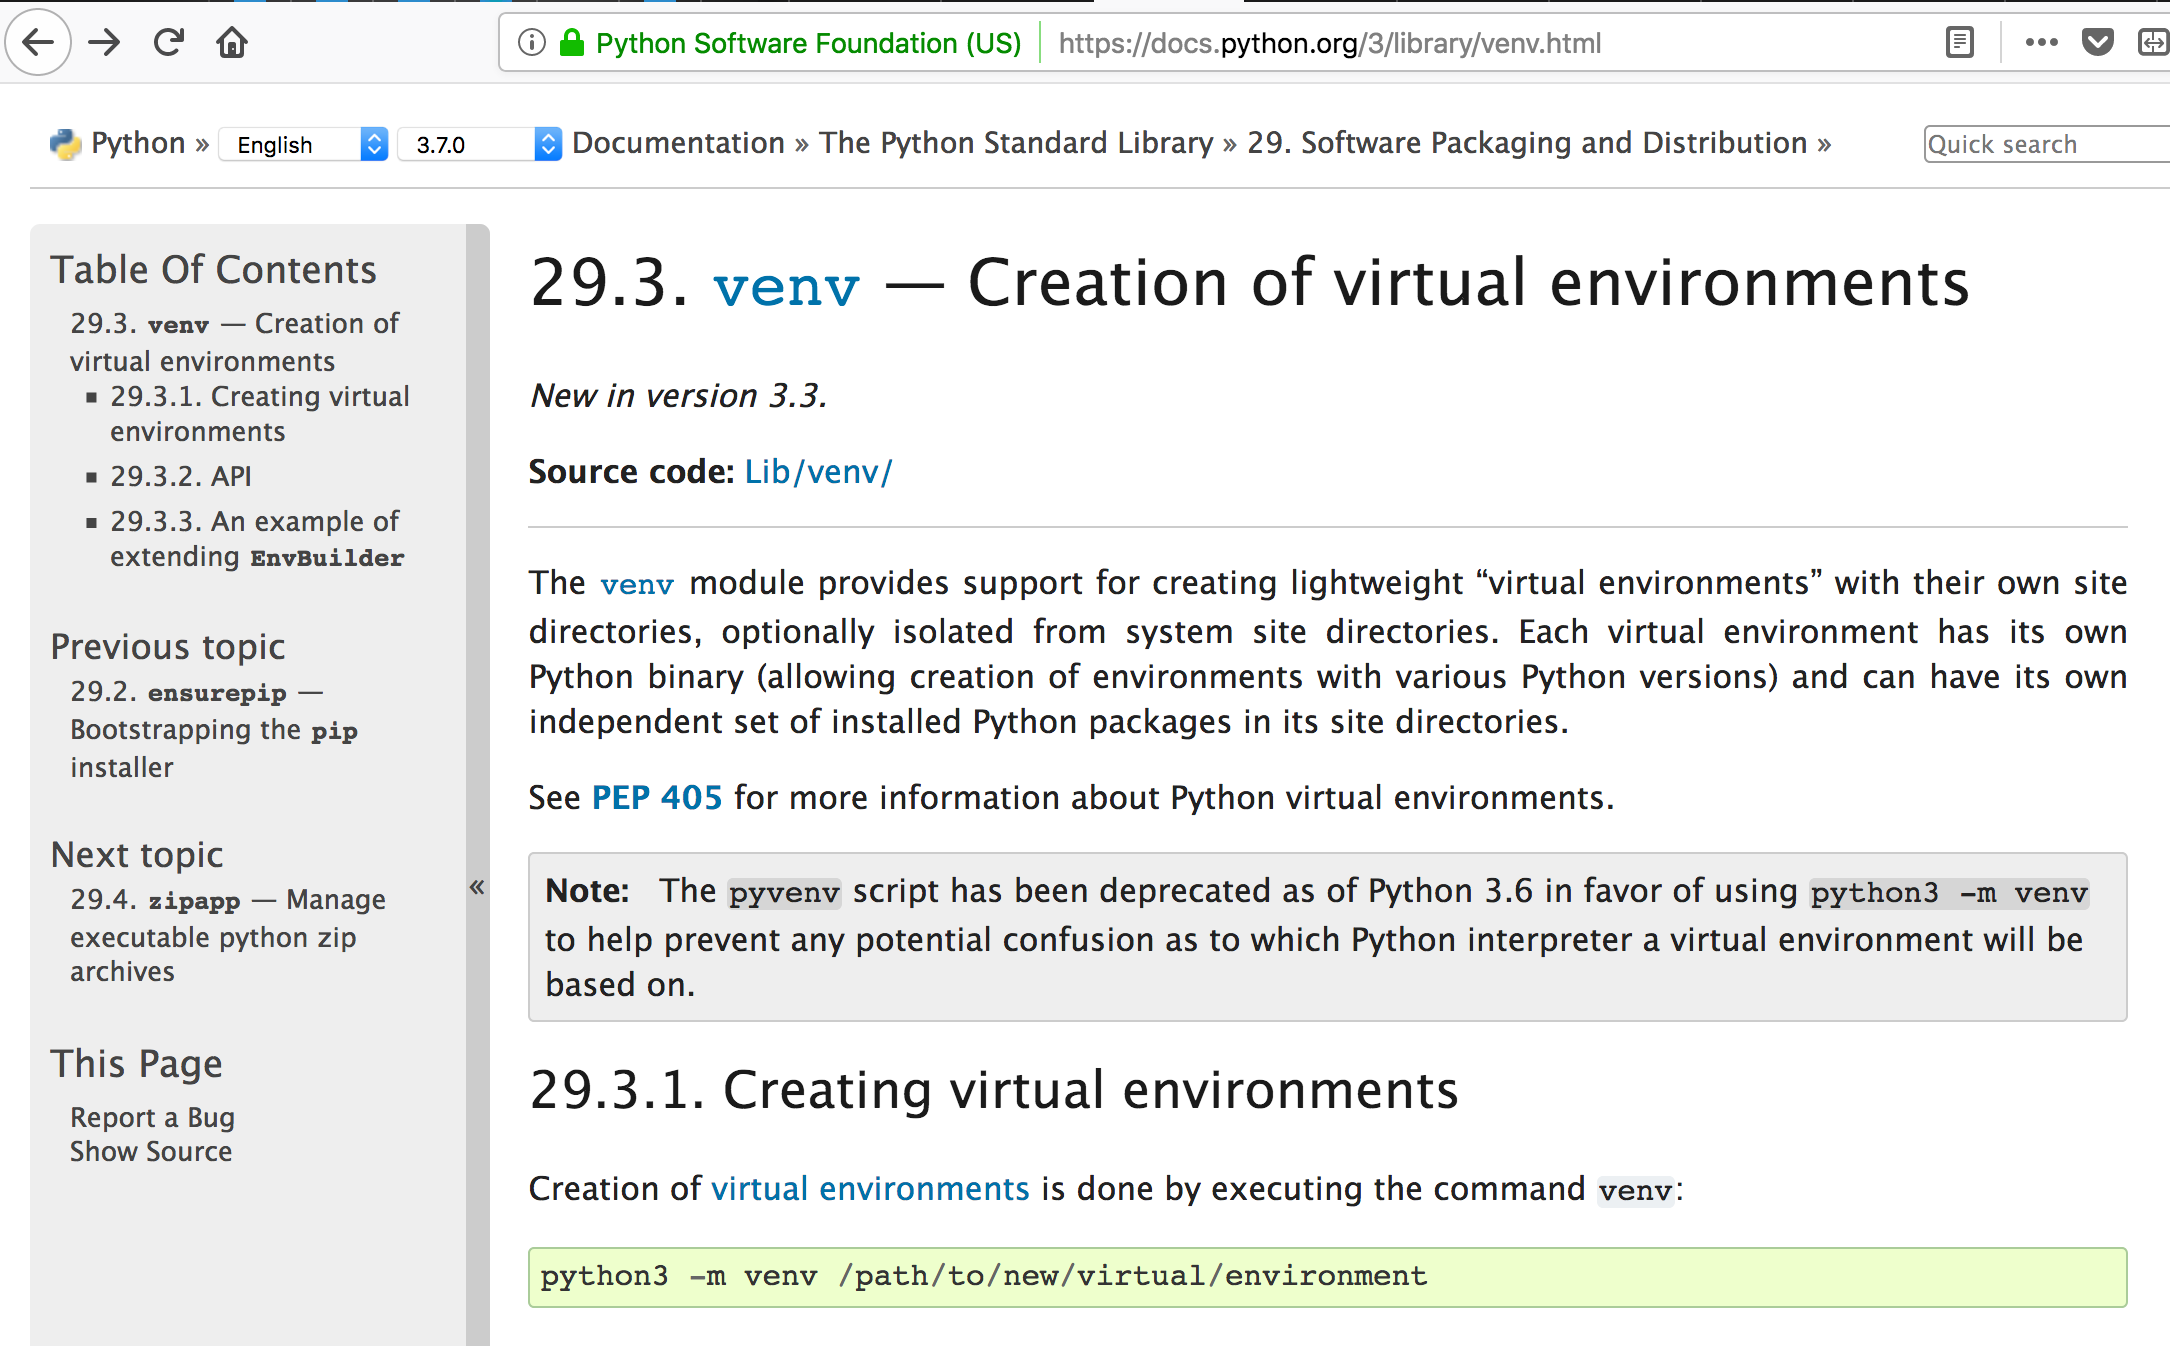
\includegraphics[width=12cm]{venv}}}
\end{frame}

\begin{frame}[fragile]{\texttt{venv}}
  \begin{itemize}
    \item virtual environments (ambientes virtuais)
    \item Não confundir com máquina virtual
    \item Ambientes leves isolados com cópias próprias dos binários
    \item Isola dependências entre projetos
    \item Isola o ambiente do python usado pelo sistema
  \end{itemize}
\end{frame}

\begin{frame}[fragile]{\texttt{venv}}
\begin{alltt}
\$ python -m venv .venv
\$ source ./.venv/bin/activate
(.venv) pppipam y\$
\end{alltt}
\end{frame}

\begin{frame}[fragile]{\href{https://packaging.python.org/}{Python Packaging User Guide}}
  \hspace*{-.5cm}\centering{\href{https://packaging.python.org/}{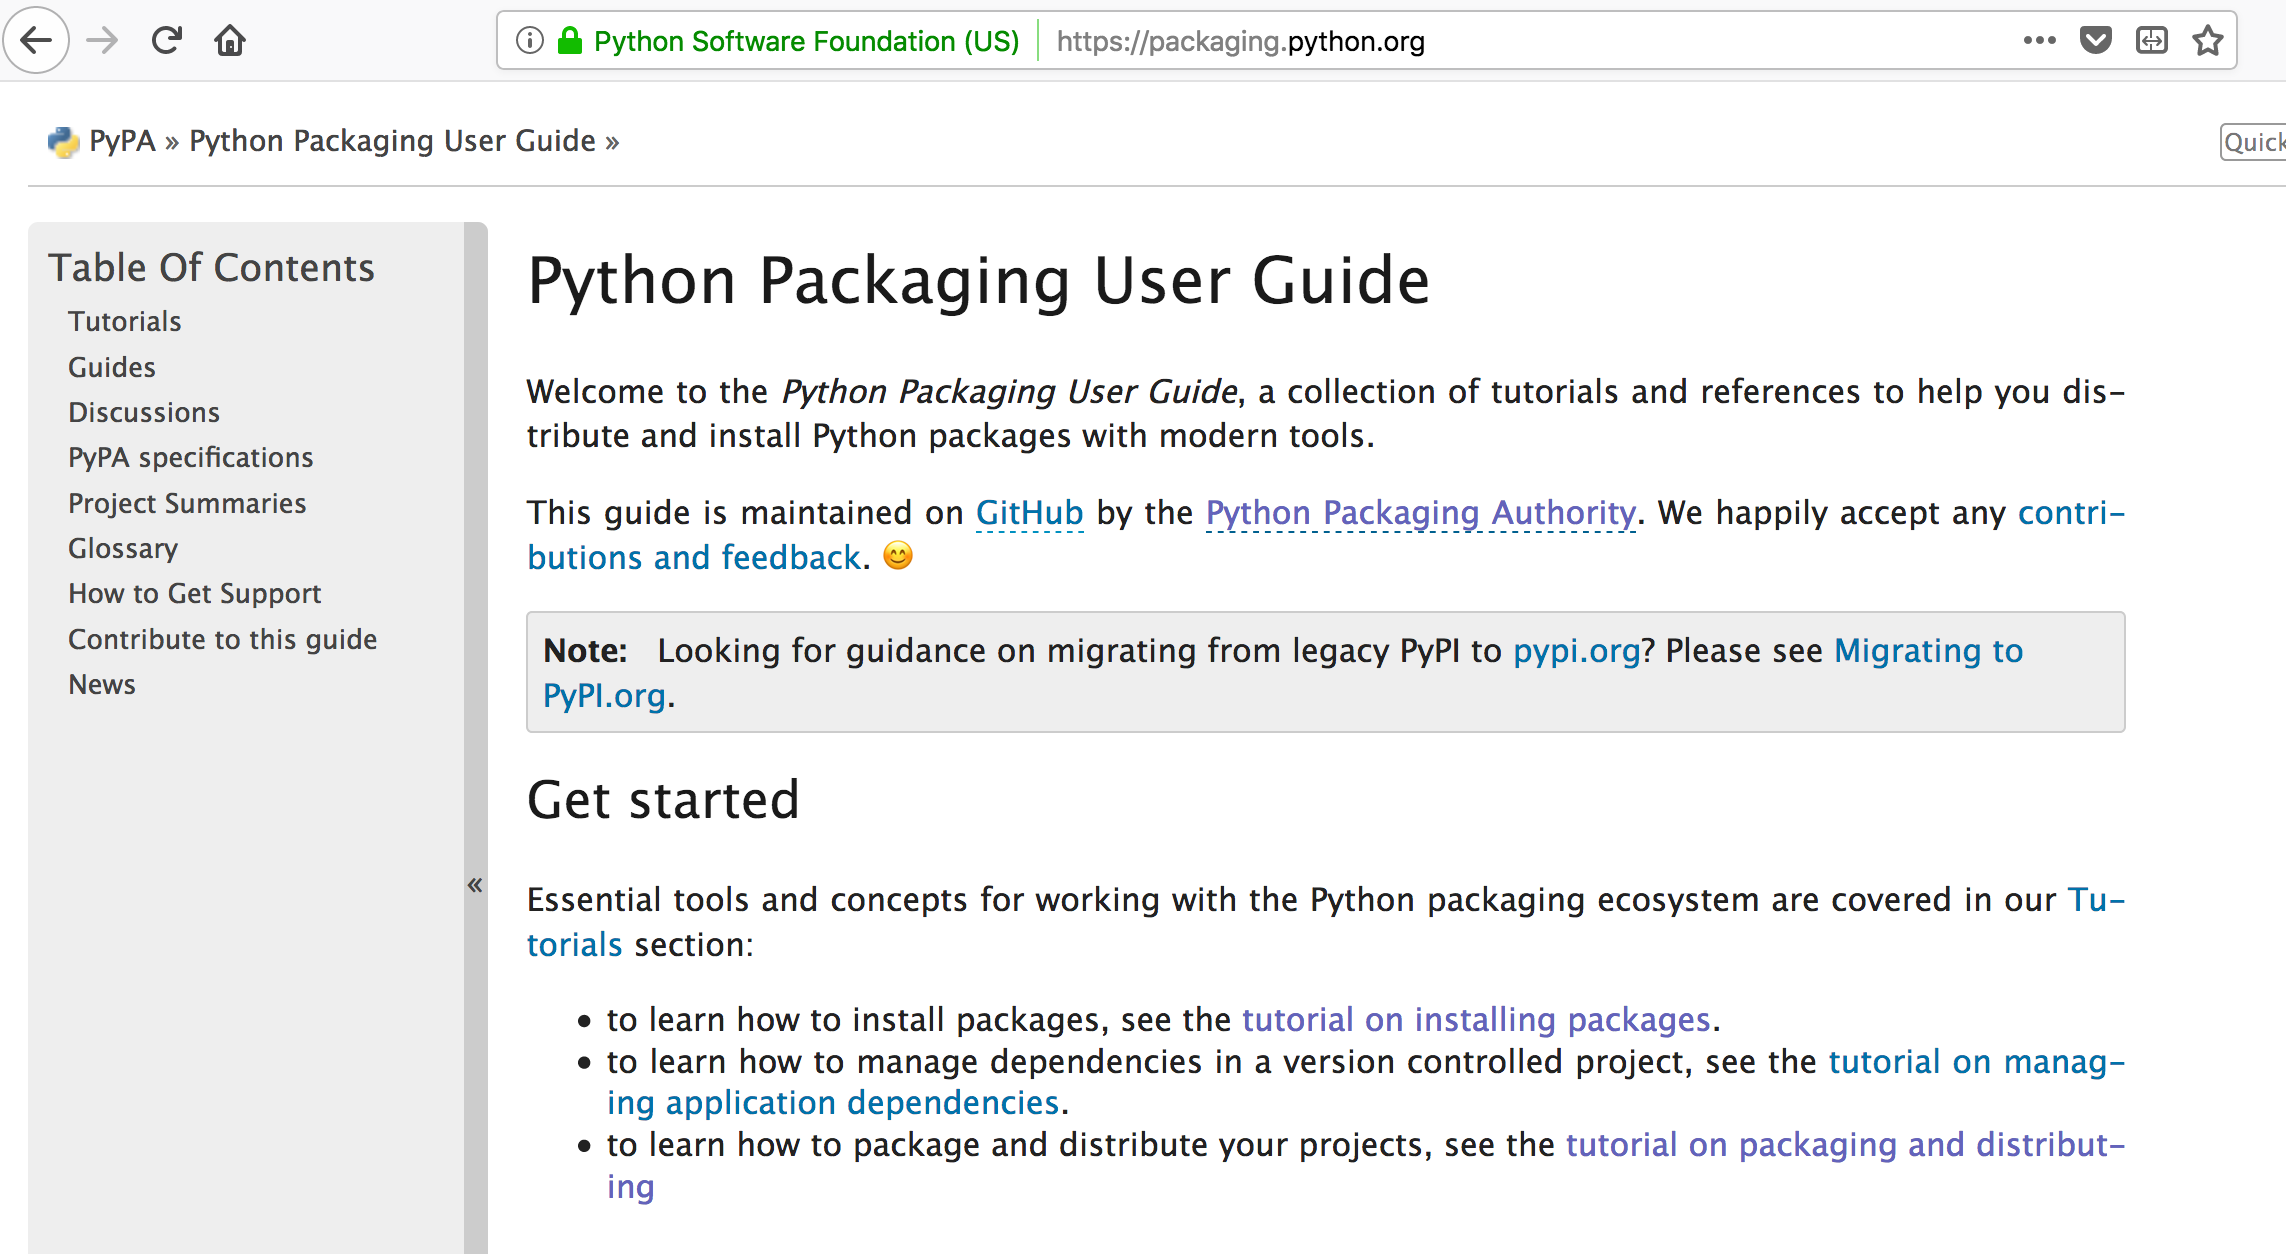
\includegraphics[width=12cm]{packaging}}}
\end{frame}

\begin{frame}[fragile]{\href{https://packaging.python.org/tutorials/packaging-projects/}{Packaging Python Projects}}
  \hspace*{-.5cm}\centering{\href{https://packaging.python.org/tutorials/packaging-projects/}{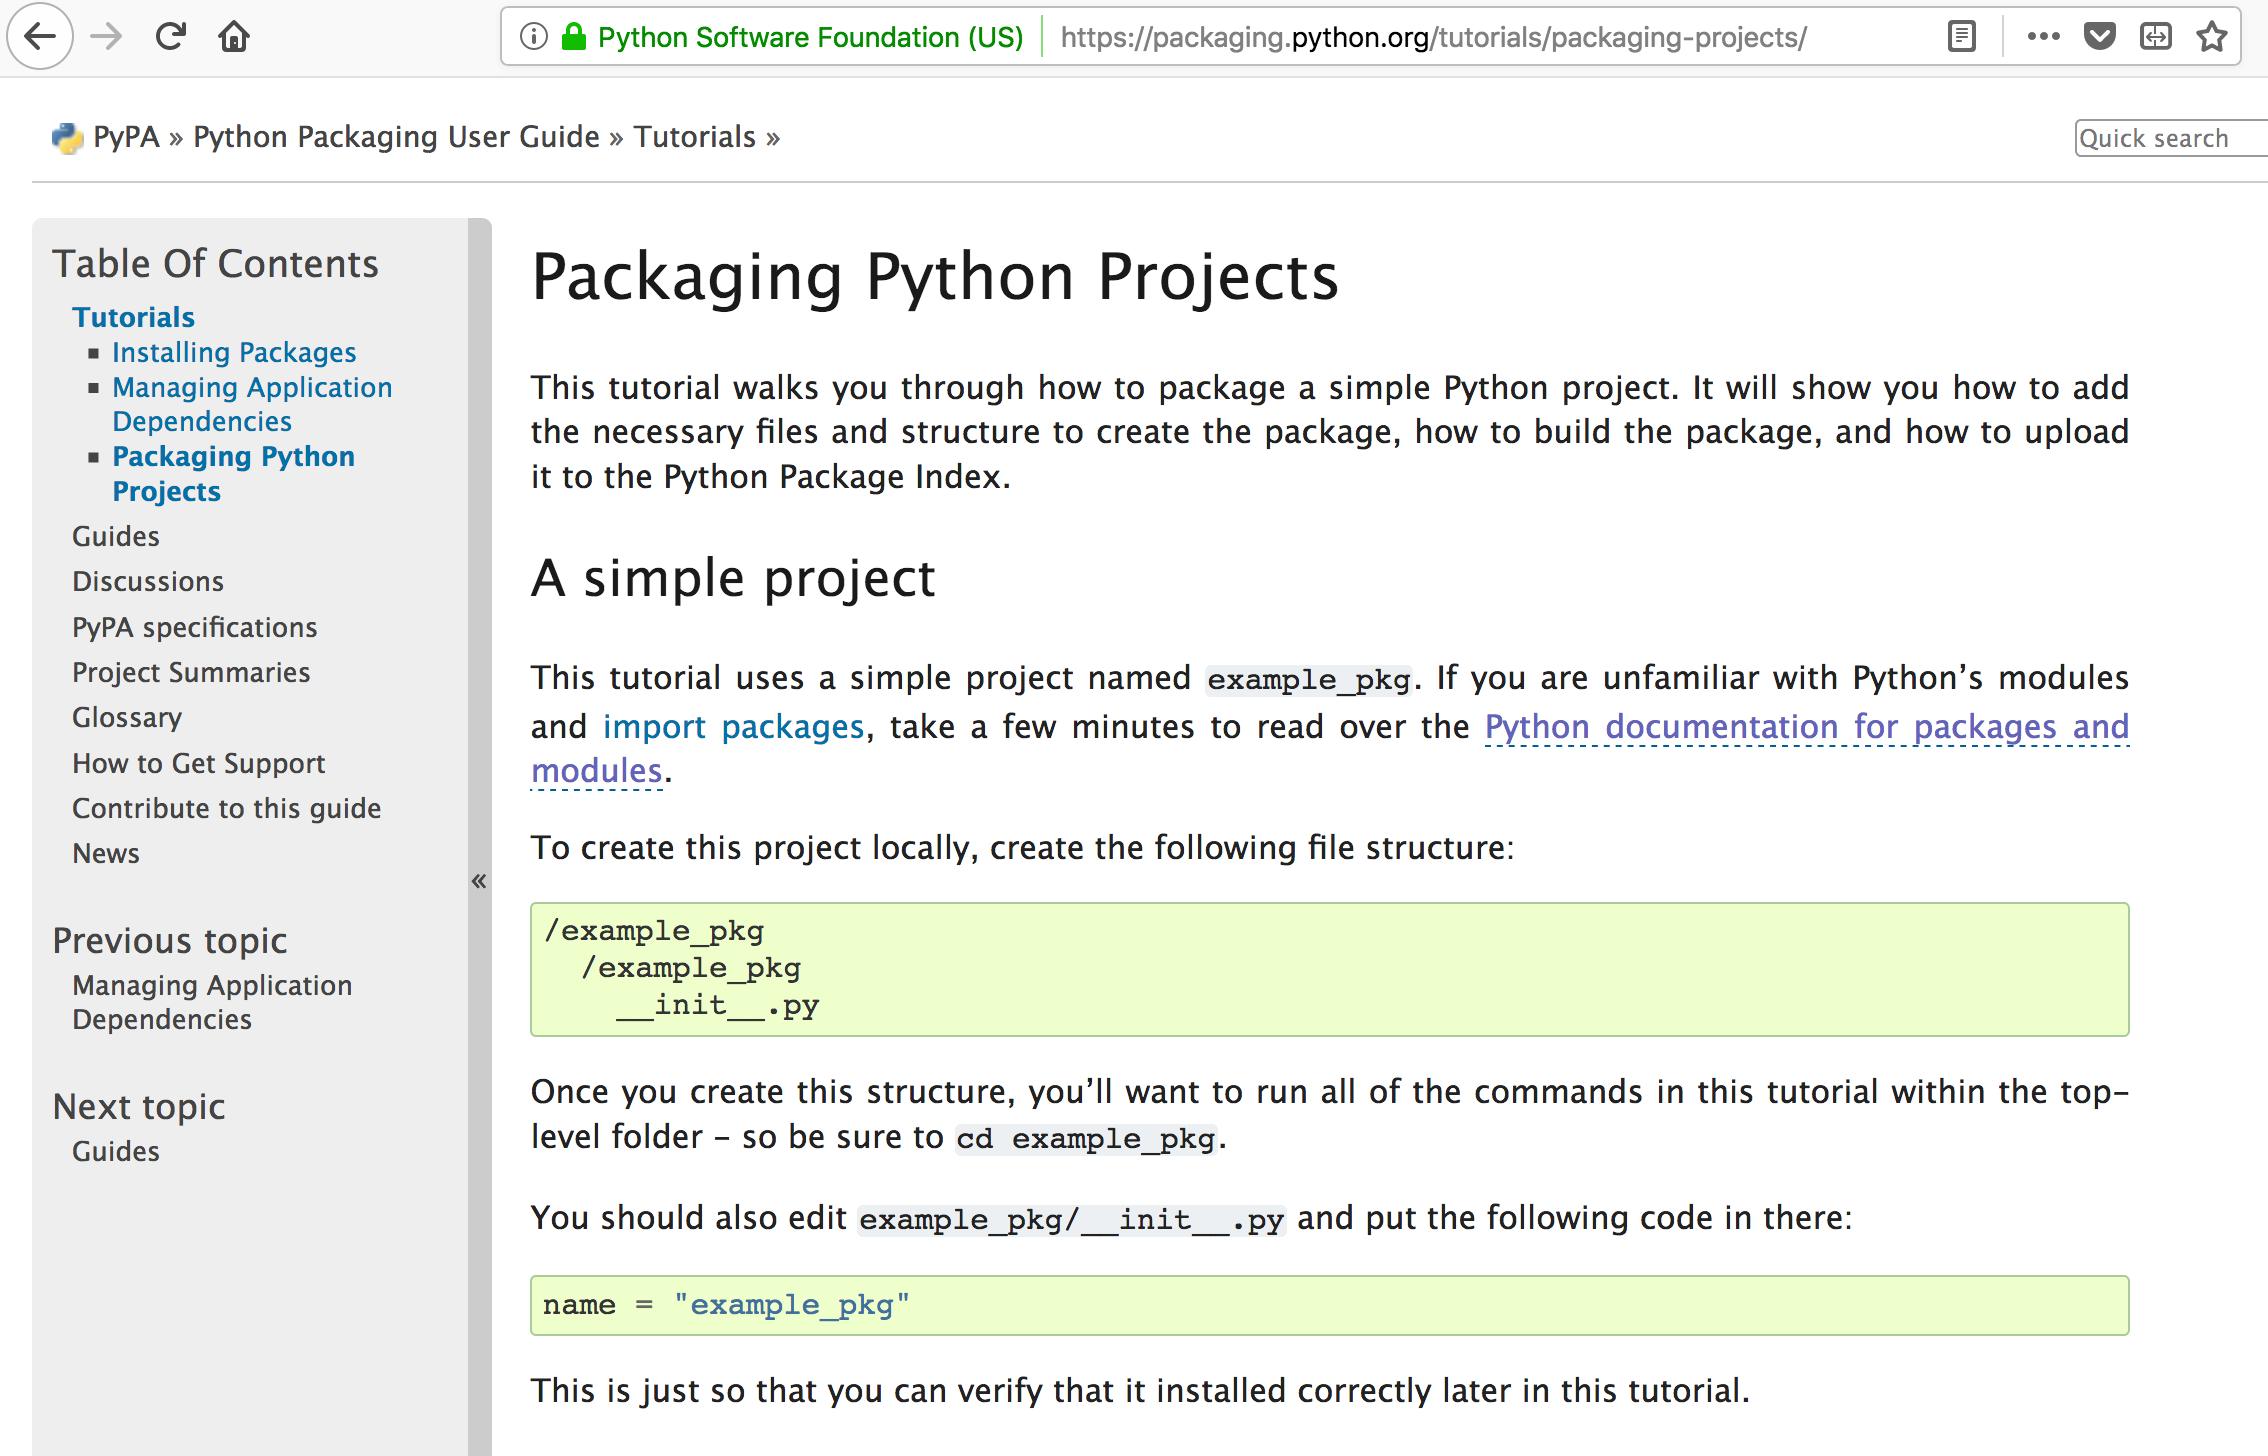
\includegraphics[width=12cm]{packaging_projects}}}
\end{frame}

\begin{frame}[fragile]{Estrutura de mínima pelo tutorial}
\begin{alltt}
.
└── example_pkg
    ├── LICENSE
    ├── README.md
    ├── example_pkg
    │   └── __init__.py
    └── setup.py
\end{alltt}
\end{frame}


\begin{frame}[fragile]{Estrutura inicial usada no PPPIPAM}
\begin{alltt}
.
└── pppipam
    ├── LICENSE
    ├── README.md
    ├── pppipam
    │   └── __init__.py
    └── tests
        └── __init__.py
\end{alltt}
\end{frame}

\begin{frame}[fragile]{Test Driven Development (TDD)}
  \hspace*{-.5cm}\centering{\href{http://tdd.caelum.com.br/}{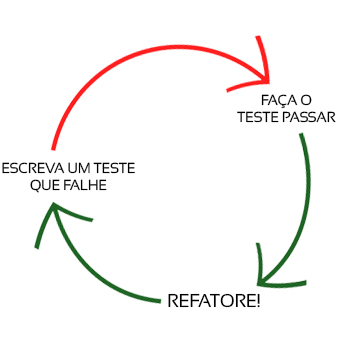
\includegraphics[width=6cm]{ciclo}}}

  \begin{flushright}
  \tiny{\vspace*{.25cm}
    Imagem obtida de \url{http://tdd.caelum.com.br/}}
  \end{flushright}
\end{frame}

\begin{frame}[fragile]{Dicas relacionadas a TDD (e em geral)}
  \begin{itemize}
    \item Use bastante o REPL para testar o comportamento esperado
    \item Leia com atenção os erros e falhas
    \item Gerou erro? Procure entender o que está escrito
    \item Não tenha medo de voltar alguns passos
  \end{itemize}
\end{frame}

\begin{frame}[fragile]{Exemplo de \texttt{TestCase} do \texttt{unittest}}
\begin{alltt}\scriptsize
import dataclass
import unittest

from pppipam.pppipam import AddressSpace

class AddressSpace_dataclass_TestCase(unittest.TestCase):
    """Tests related to verify if AddressSpace is a dataclass."""
    def test_address_space_is_dataclass(self):
        """Validate if AddressSpace is a dataclass."""
        self.assertTrue(
            dataclasses.is_dataclass(AddressSpace),
            "AddressSpace expected to be a dataclass"
        )
\end{alltt}
\end{frame}


\begin{frame}[fragile]{\href{https://docs.python.org/3/library/pydoc.html}{\texttt{pydoc}}}
Exibe \texttt{docstrings} ao acionar a buitin \texttt{help}. 

\begin{alltt}
>>> help(helpers.clean_network)
\end{alltt}
\end{frame}


\begin{frame}[fragile]{\href{https://docs.python.org/3/library/pydoc.html}{\texttt{pydoc}}}
\begin{alltt}\tiny
Help on function clean_network in module pppipam.helpers:

clean_network(network_parameter: Union[str, ipaddress.IPv4Network, ipaddress.IPv6Network]) -> Union[ipaddress.IPv4Network, ipaddress.IPv6Network, NoneType]
    Process given parameter as a Network instance.

    If parameter results into a valid IPv4 or IPv6 network,
    it respectively returns IPv4Network or IPv6Network.
    Otherwise, returns None.

    >>> clean_network("invalid network")
    >>> clean_network("10.0.0.0/8")
    IPv4Network('10.0.0.0/8')
    >>> clean_network("fe80::/64")
    IPv6Network('fe80::/64')

    Args:
        network_parameter: value to be processed as an IP network.

    Returns:
        IPv4Network instance, IPv6Network instance or None.
\end{alltt}
\end{frame}

\begin{frame}[fragile]{\href{https://docs.python.org/3/library/doctest.html}{\texttt{doctest}}}
  \begin{itemize}
    \item Fornece exemplo executável no REPL
    \item Diferente do propósito do unittest: apresenta exatamente o resultado esperado após execução
  \end{itemize}
\end{frame}

\begin{frame}[fragile]{Exemplo de integração \texttt{unittest} e \texttt{doctest}}
\begin{alltt}\scriptsize
import doctest
import unittest

from pppipam import helpers, pppipam


def load_tests(loader, tests, ignore):
    """Base example provided in doctest documentation."""

    tests.addTests(doctest.DocTestSuite(helpers))
    tests.addTests(doctest.DocTestSuite(pppipam))
    return tests
\end{alltt}
\end{frame}


\begin{frame}[fragile]{Exceptions}
\begin{alltt}\scriptsize
class StrictSupernetError(Exception):
    """Error related to supernet missing or present."""
    pass

class SameDelegationAsNewError(Exception):
    """Attempt to insert already existing delegated network."""
    pass
\end{alltt}
\end{frame}

\begin{frame}[fragile]{\href{https://packaging.python.org/}{Python Packaging User Guide}}
  \hspace*{-.5cm}\centering{\href{https://packaging.python.org/}{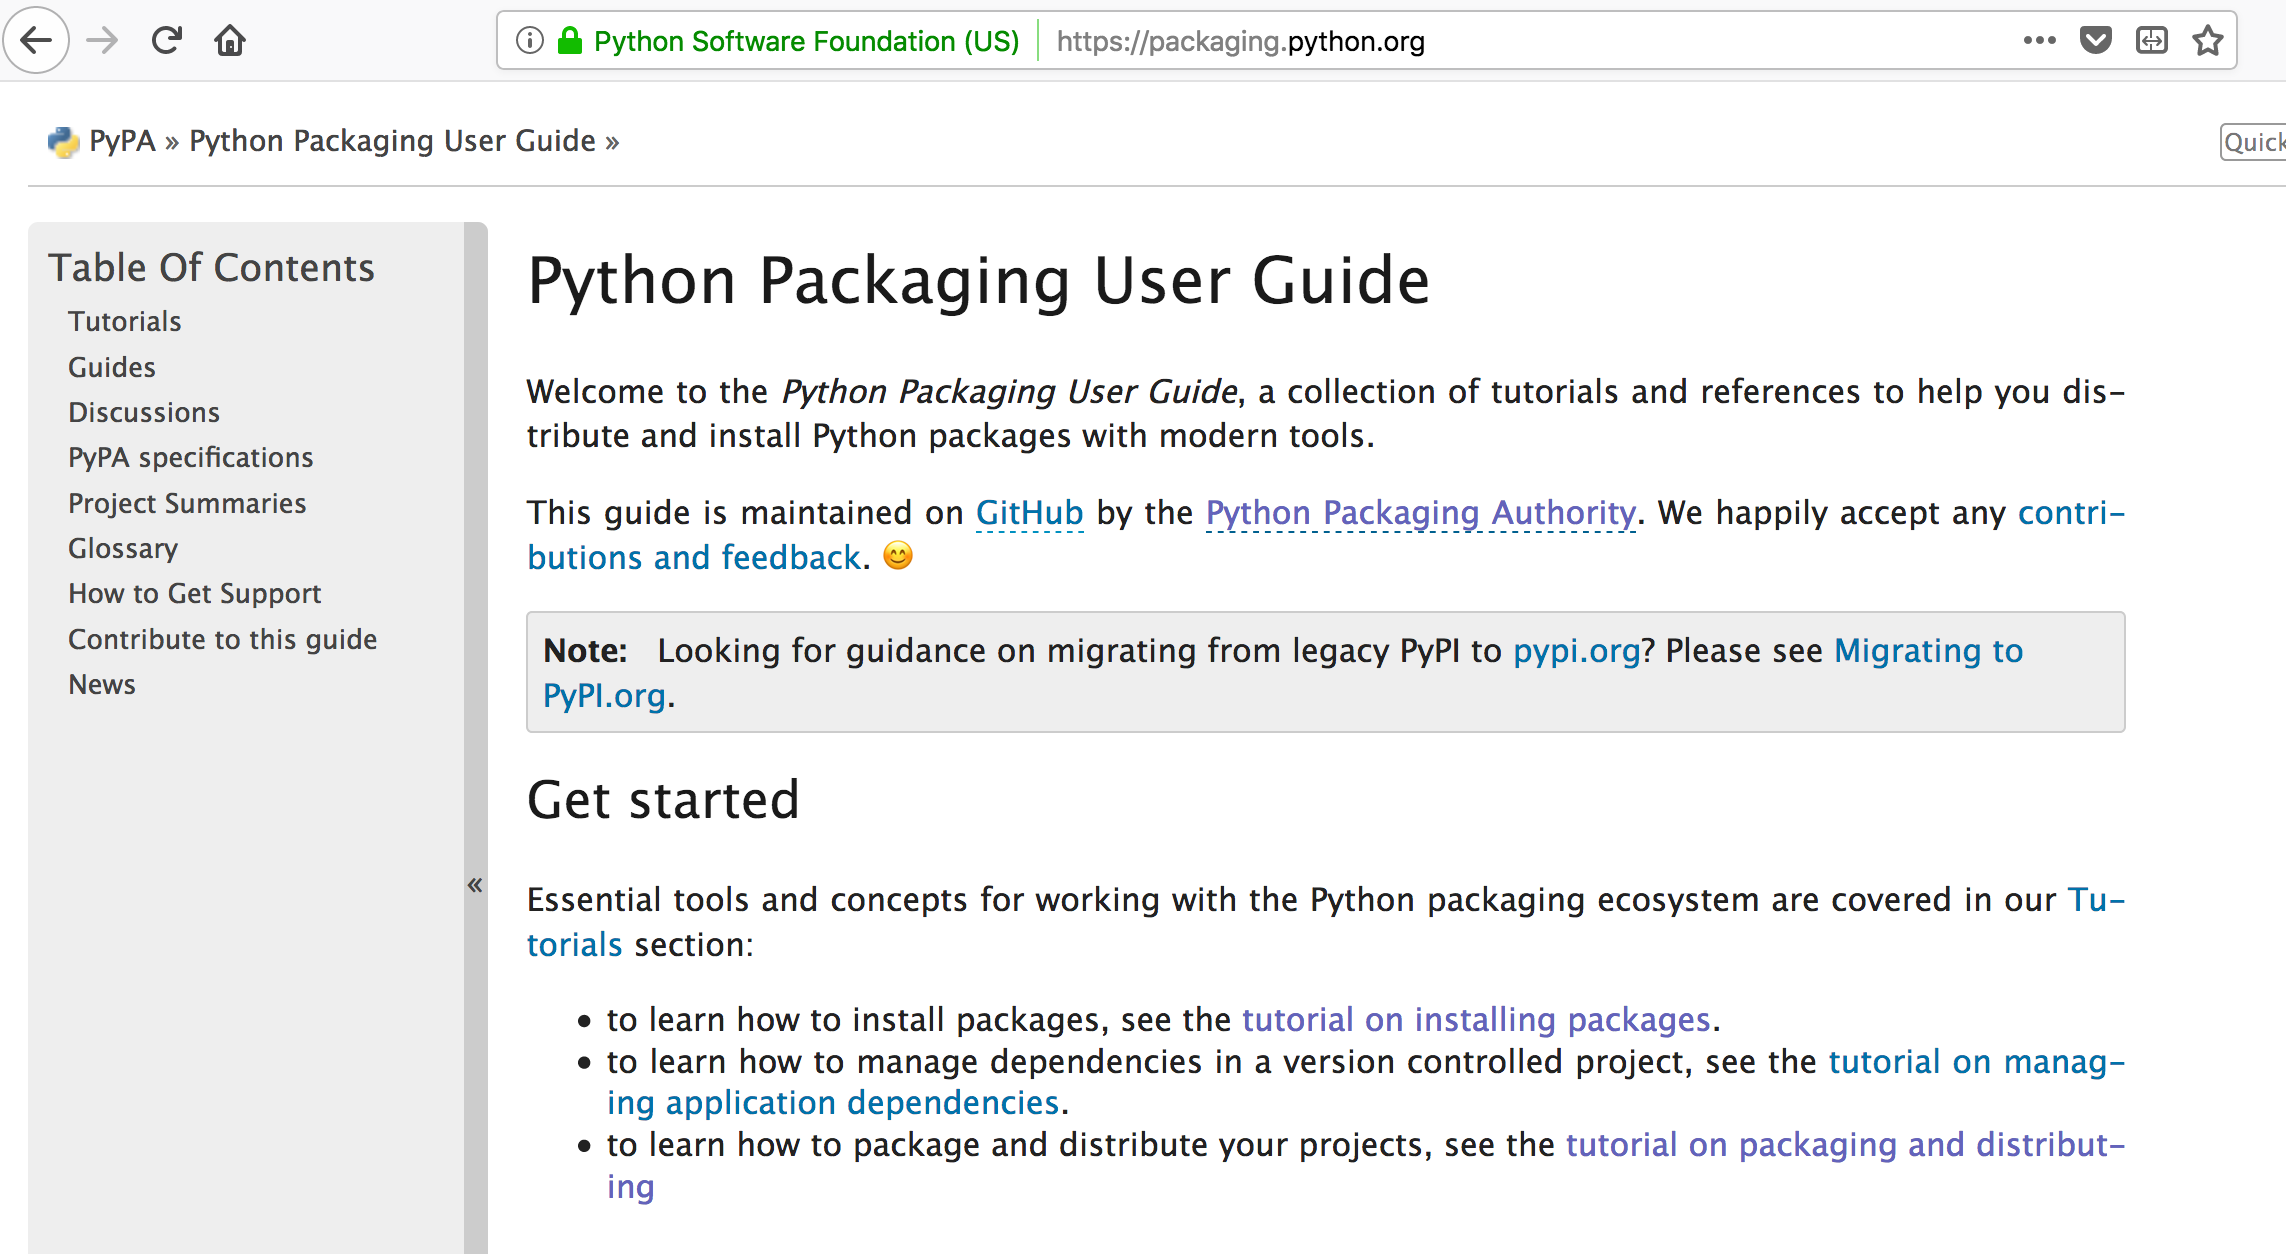
\includegraphics[width=12cm]{packaging}}}
\end{frame}

\begin{frame}[fragile]{\href{https://packaging.python.org/tutorials/packaging-projects/}{Packaging Python Projects}}
  \hspace*{-.5cm}\centering{\href{https://packaging.python.org/tutorials/packaging-projects/}{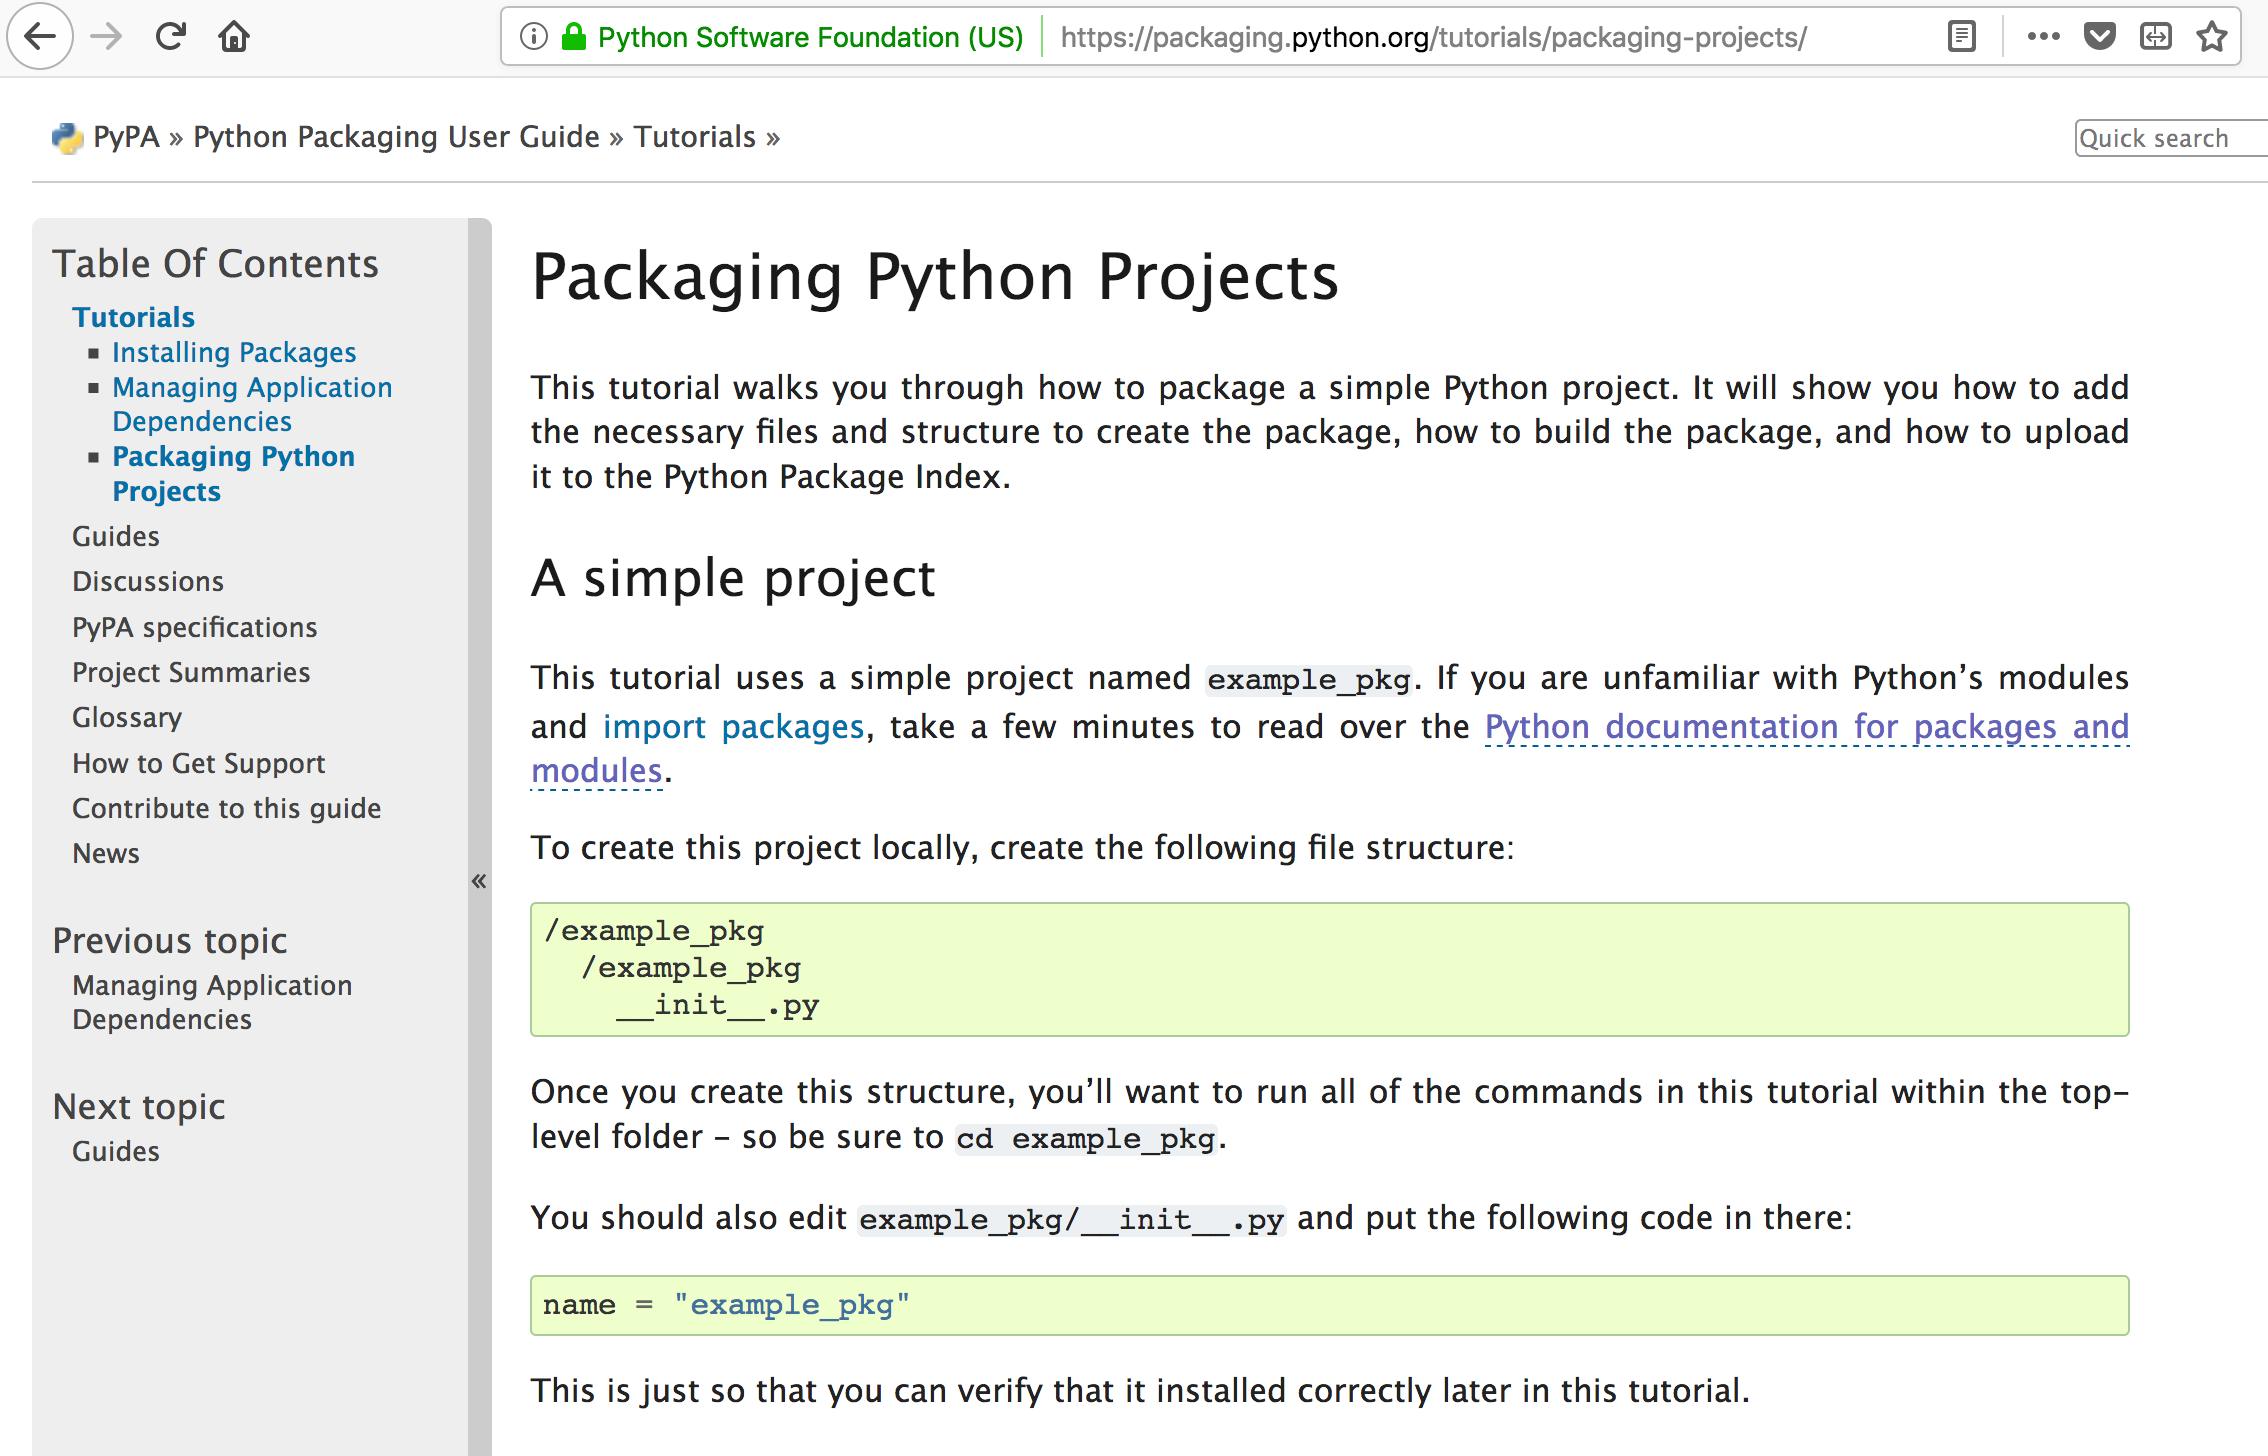
\includegraphics[width=12cm]{packaging_projects}}}
\end{frame}

\begin{frame}[fragile]{\href{https://github.com/pypa/sampleproject}{pypa/sampleproject}}
  \hspace*{-.5cm}\centering{\href{https://github.com/pypa/sampleproject}{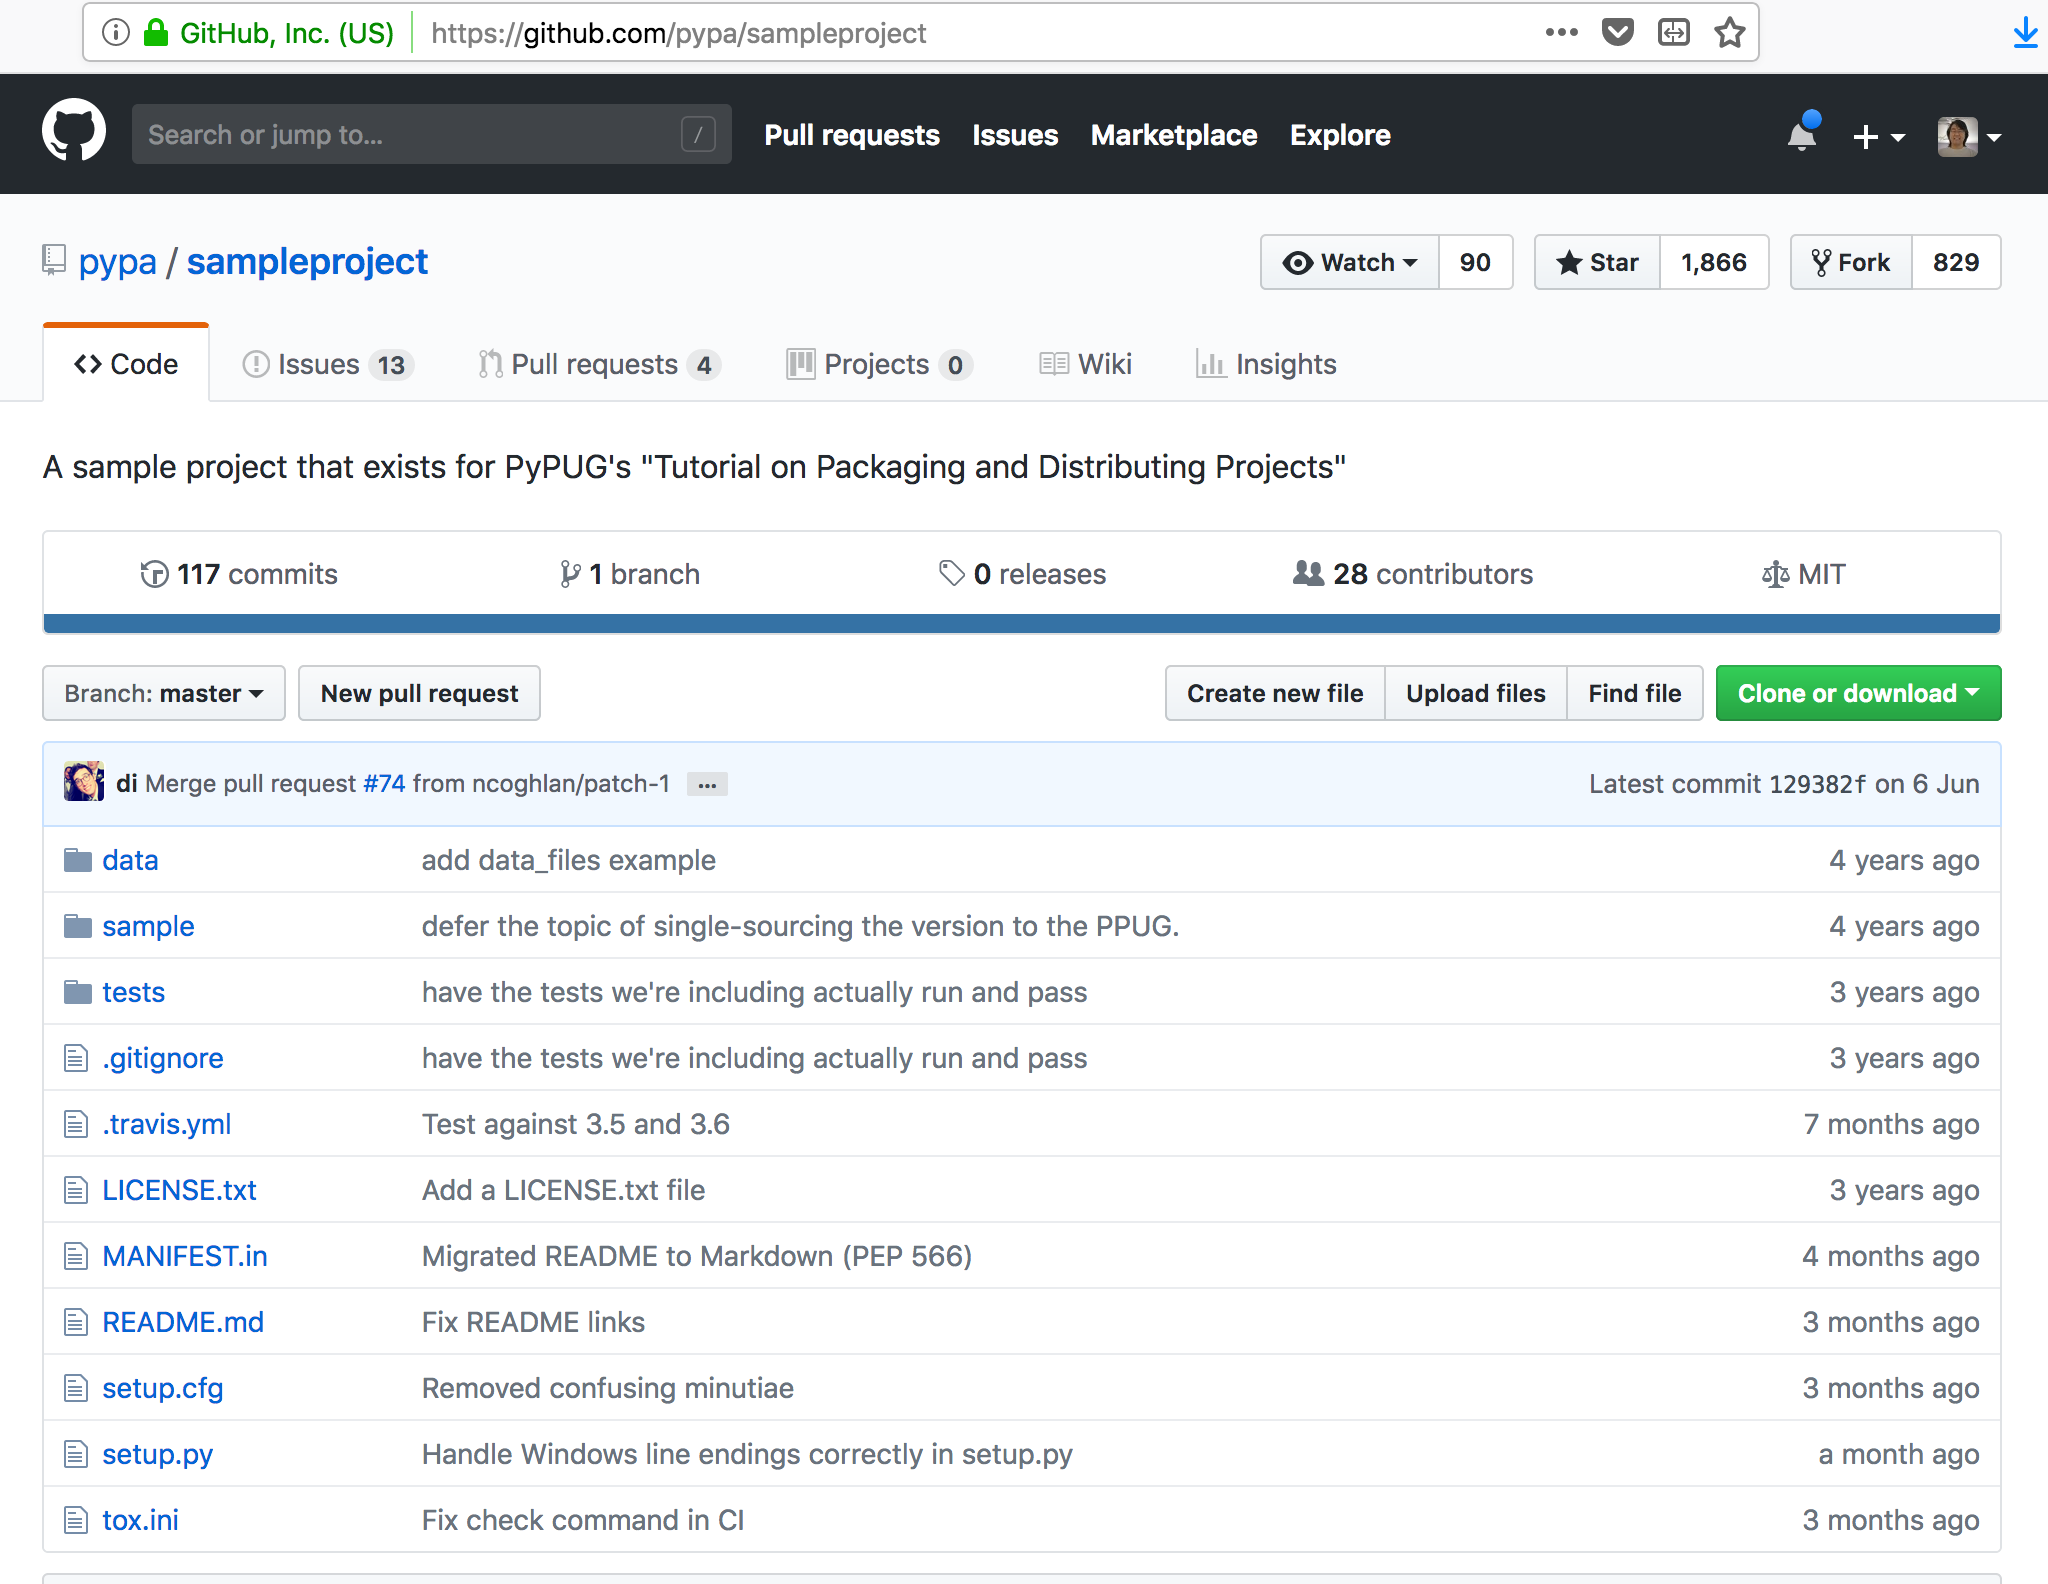
\includegraphics[width=12cm]{sample}}}
\end{frame}

\begin{frame}[fragile]{Estrutura final usada no PPPIPAM}
\begin{alltt}\scriptsize
.
└── pppipam
    ├── CHANGELOG.rst
    ├── CONTRIBUTORS.rst
    ├── LICENSE
    ├── README.md
    ├── setup.py
    ├── setup.cfg
    ├── pppipam
    │   ├── __init__.py
    │   ├── helpers.py
    │   └── pppipam.py
        └── test_strictness.py
    .
    .
    .
\end{alltt}
\end{frame}

\begin{frame}[fragile]{Estrutura final usada no PPPIPAM}
\begin{alltt}\scriptsize
.
└── pppipam
    .
    .
    .
    └── tests
        ├── __init__.py
        ├── test_dataclass.py
        ├── test_description.py
        ├── test_helpers.py
        ├── test_pppipam_doctests.py
        └── test_strictness.py
\end{alltt}
\end{frame}

\begin{frame}[fragile]{Empacotamento}
  \begin{itemize}
    \item Source distribution
    \item Wheels
      \begin{itemize}
        \item Universal Wheels (Python 2 e 3)
        \item Pure Python Wheels (Python somente 2 ou somente 3)
        \item Platform Wheels (Linux, macOS, Windows, ...)
      \end{itemize}
  \end{itemize}
\end{frame}

% TODO: arquivos

\begin{frame}[fragile]{\href{https://test.pypi.org/}{TestPyPI}}
  \hspace*{-.5cm}\centering{\href{https://test.pypi.org/}{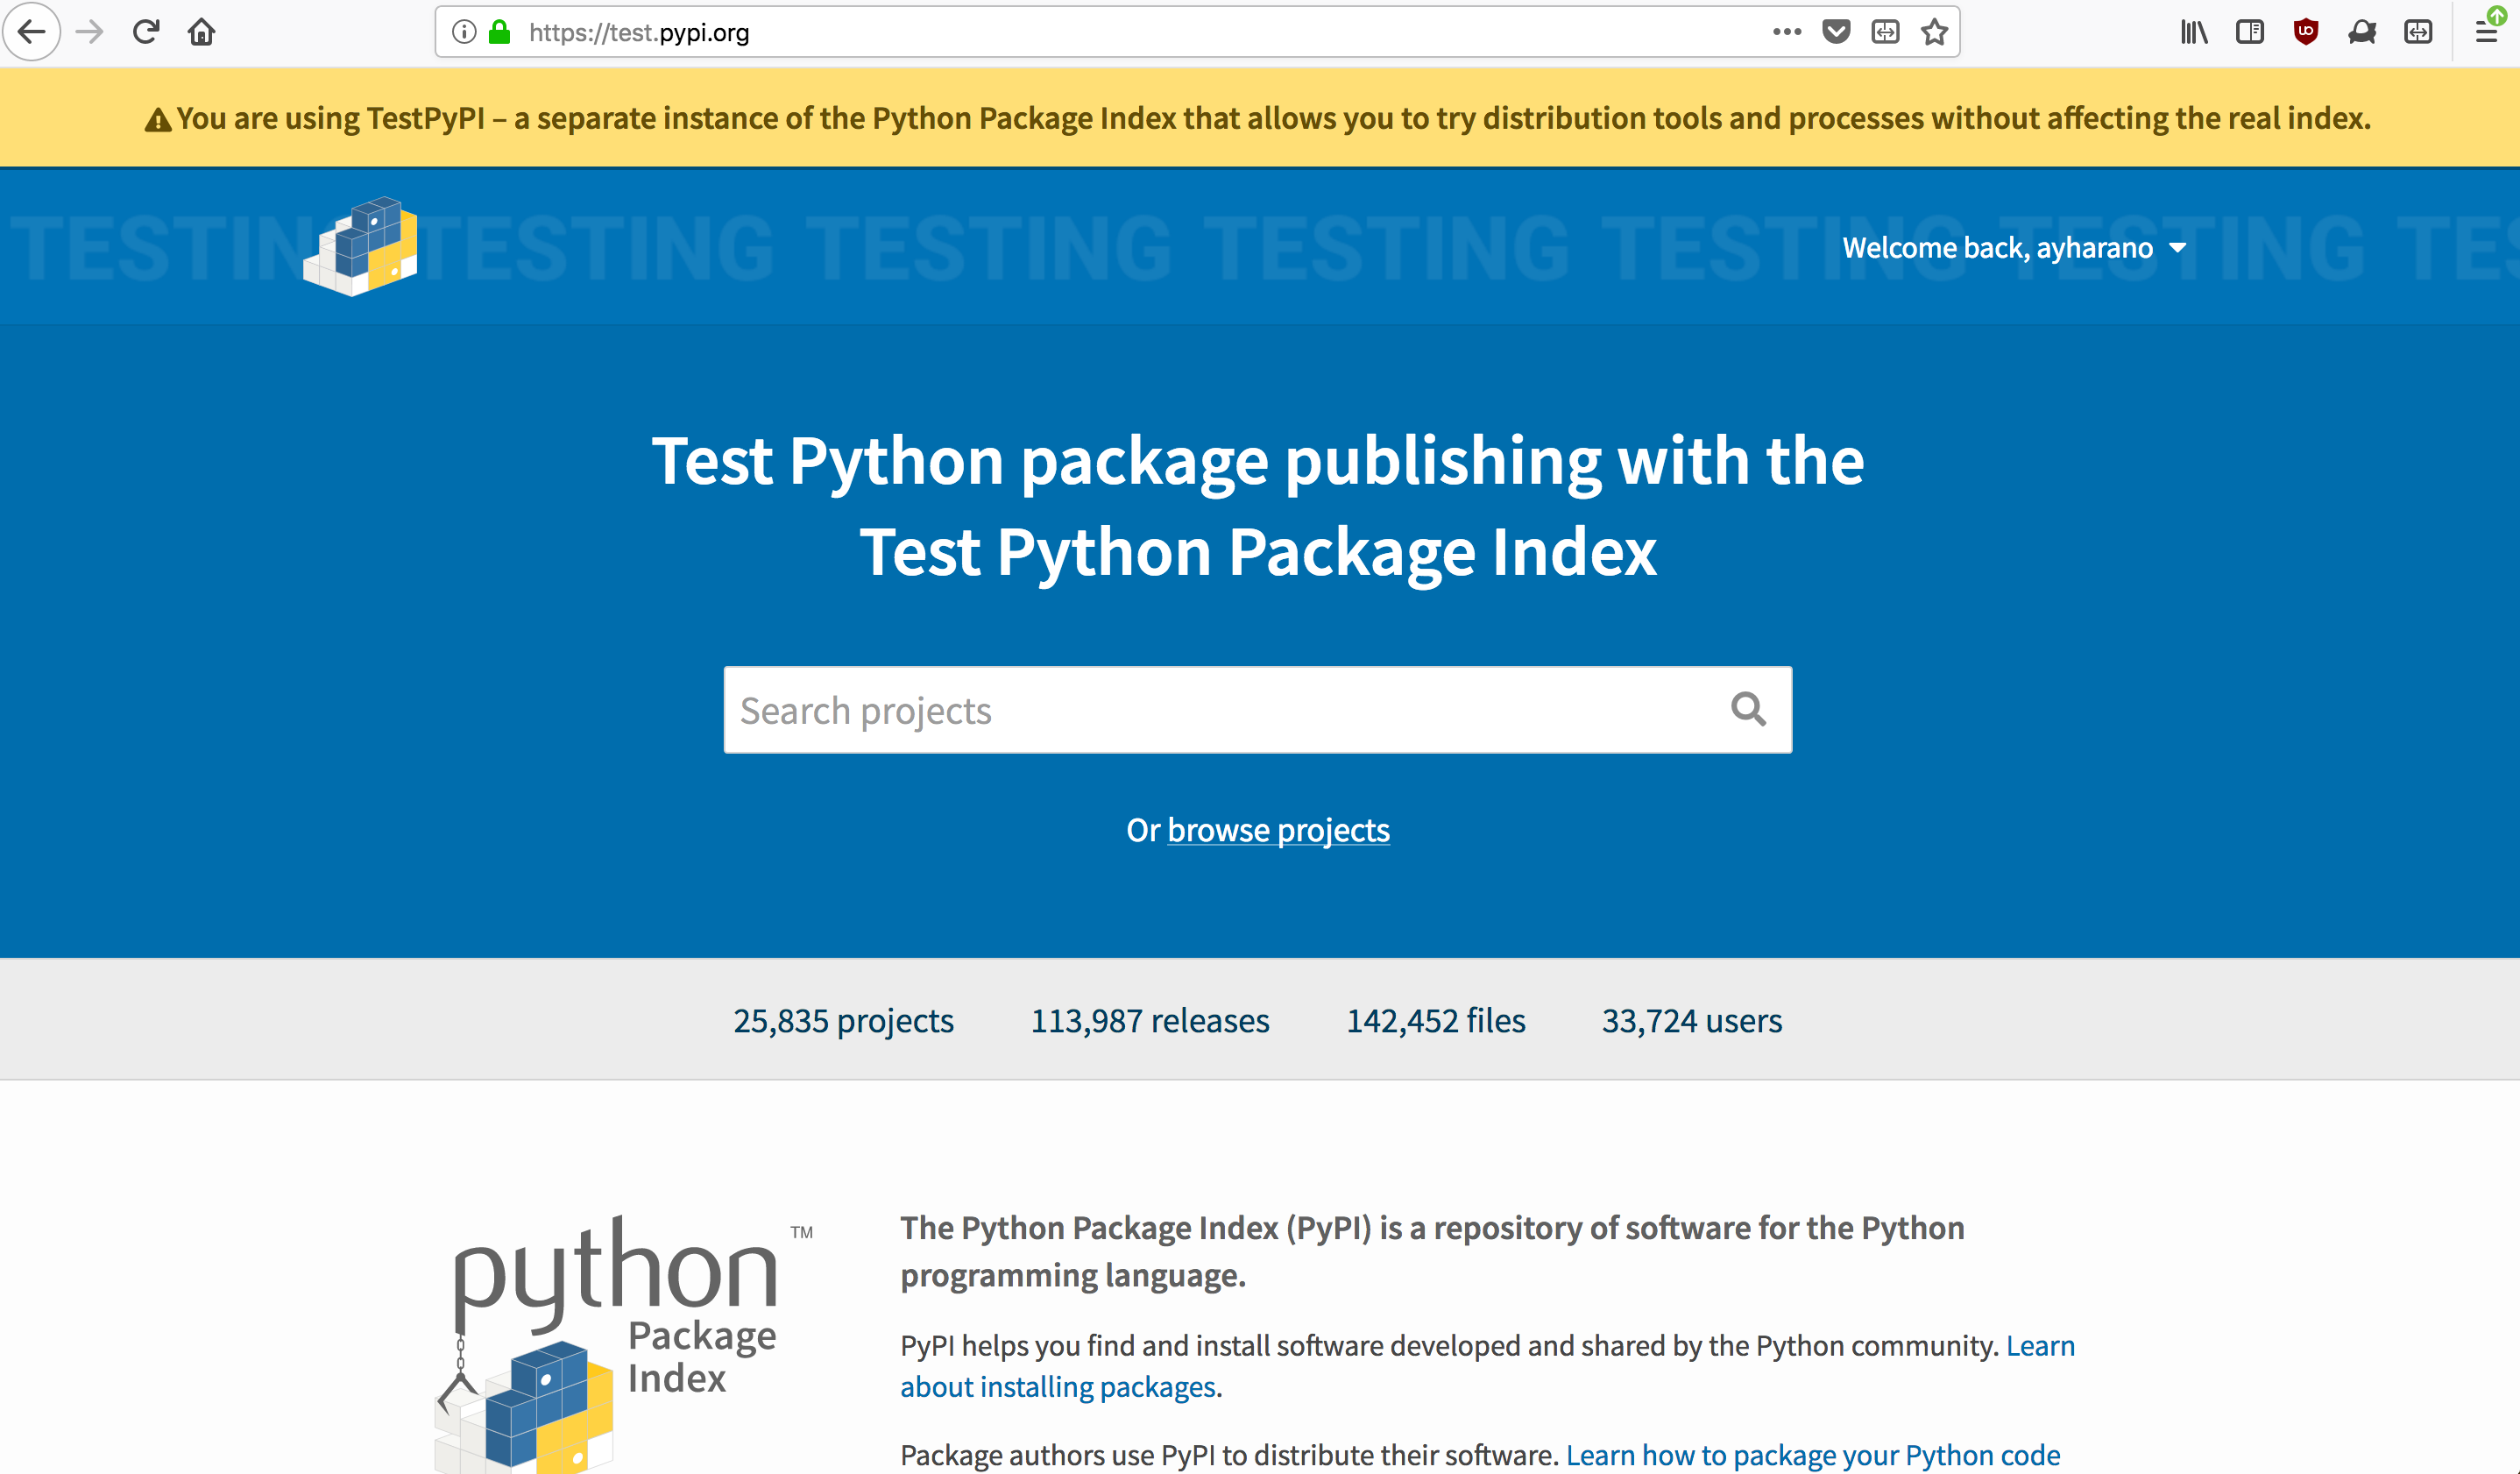
\includegraphics[width=12cm]{test_pypi}}}
\end{frame}

\begin{frame}[fragile]
\begin{alltt}\tiny
\$ python3 -m pip install \verb+\+
  --index-url https://test.pypi.org/simple/ pppipam
Looking in indexes: https://test.pypi.org/simple/
Collecting pppipam
  Downloading https://test-files.pythonhosted.org/packages/.../pppipam-0.1.0-py3-none-any.whl
Installing collected packages: pppipam
Successfully installed pppipam-0.1.0
\end{alltt}
\end{frame}

\begin{frame}[fragile]{\href{https://pypi.org/}{PyPI}}
  \hspace*{-.5cm}\centering{\href{https://pypi.org/}{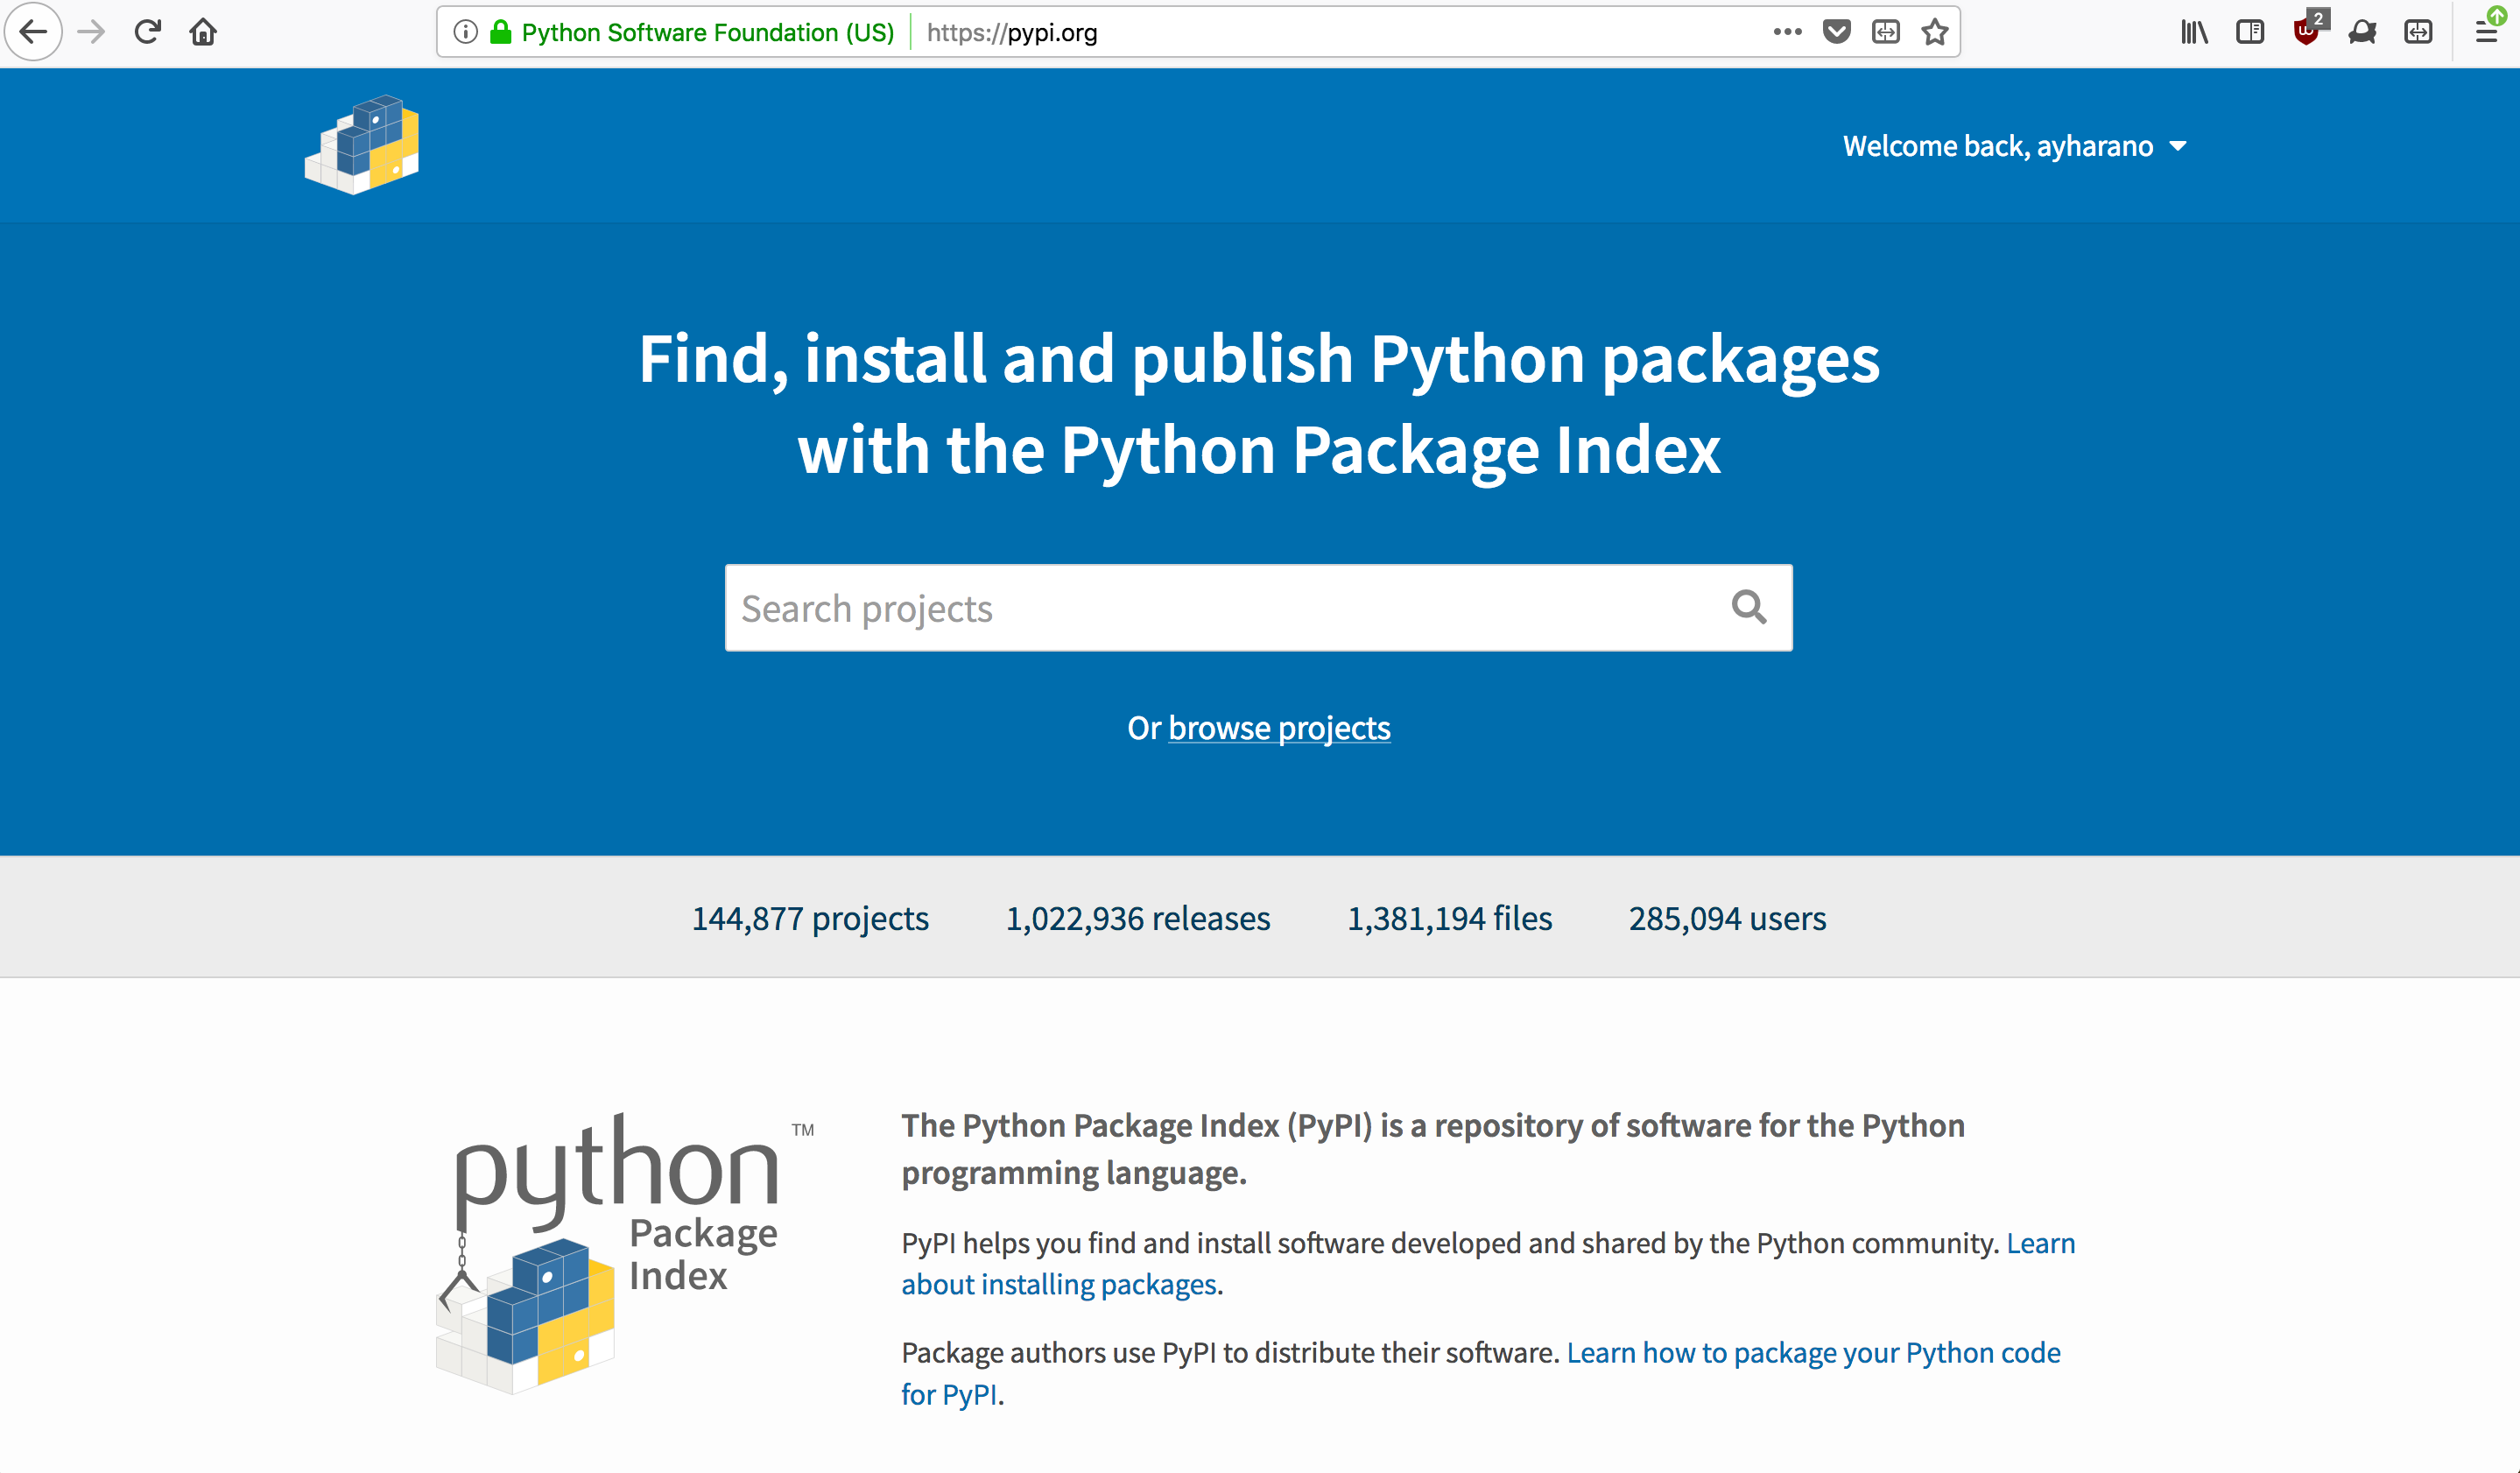
\includegraphics[width=12cm]{pypi}}}
\end{frame}

\begin{frame}[fragile]{\href{https://pypi.org/}{PyPI}}
  \href{https://pypi.org/}{PyPI}: \url{https://pypi.org/}

  \begin{itemize}
    \item Python Package Index (PyPI)
    \item Repositório padrão de software para Python
  \end{itemize}
\end{frame}

\begin{frame}[fragile]
\begin{alltt}\footnotesize
(.venv) pppipam y\$ twine upload --sign dist/*
Uploading distributions to https://upload.pypi.org/legacy/
Enter your username: ayharano
Enter your password:
Signing pppipam-0.1.0-py3-none-any.whl
Uploading pppipam-0.1.0-py3-none-any.whl
100%|█████████████| 15.0k/15.0k [00:02<00:00, 5.64kB/s]
Signing pppipam-0.1.0.tar.gz
Uploading pppipam-0.1.0.tar.gz
100%|█████████████| 15.2k/15.2k [00:01<00:00, 10.3kB/s]
(.venv) pppipam y\$
\end{alltt}
\end{frame}


\begin{frame}[fragile]{\href{https://pypi.org/project/pppipam/}{PPPIPAM}}
  \hspace*{-.5cm}\centering{\href{https://pypi.org/project/pppipam/}{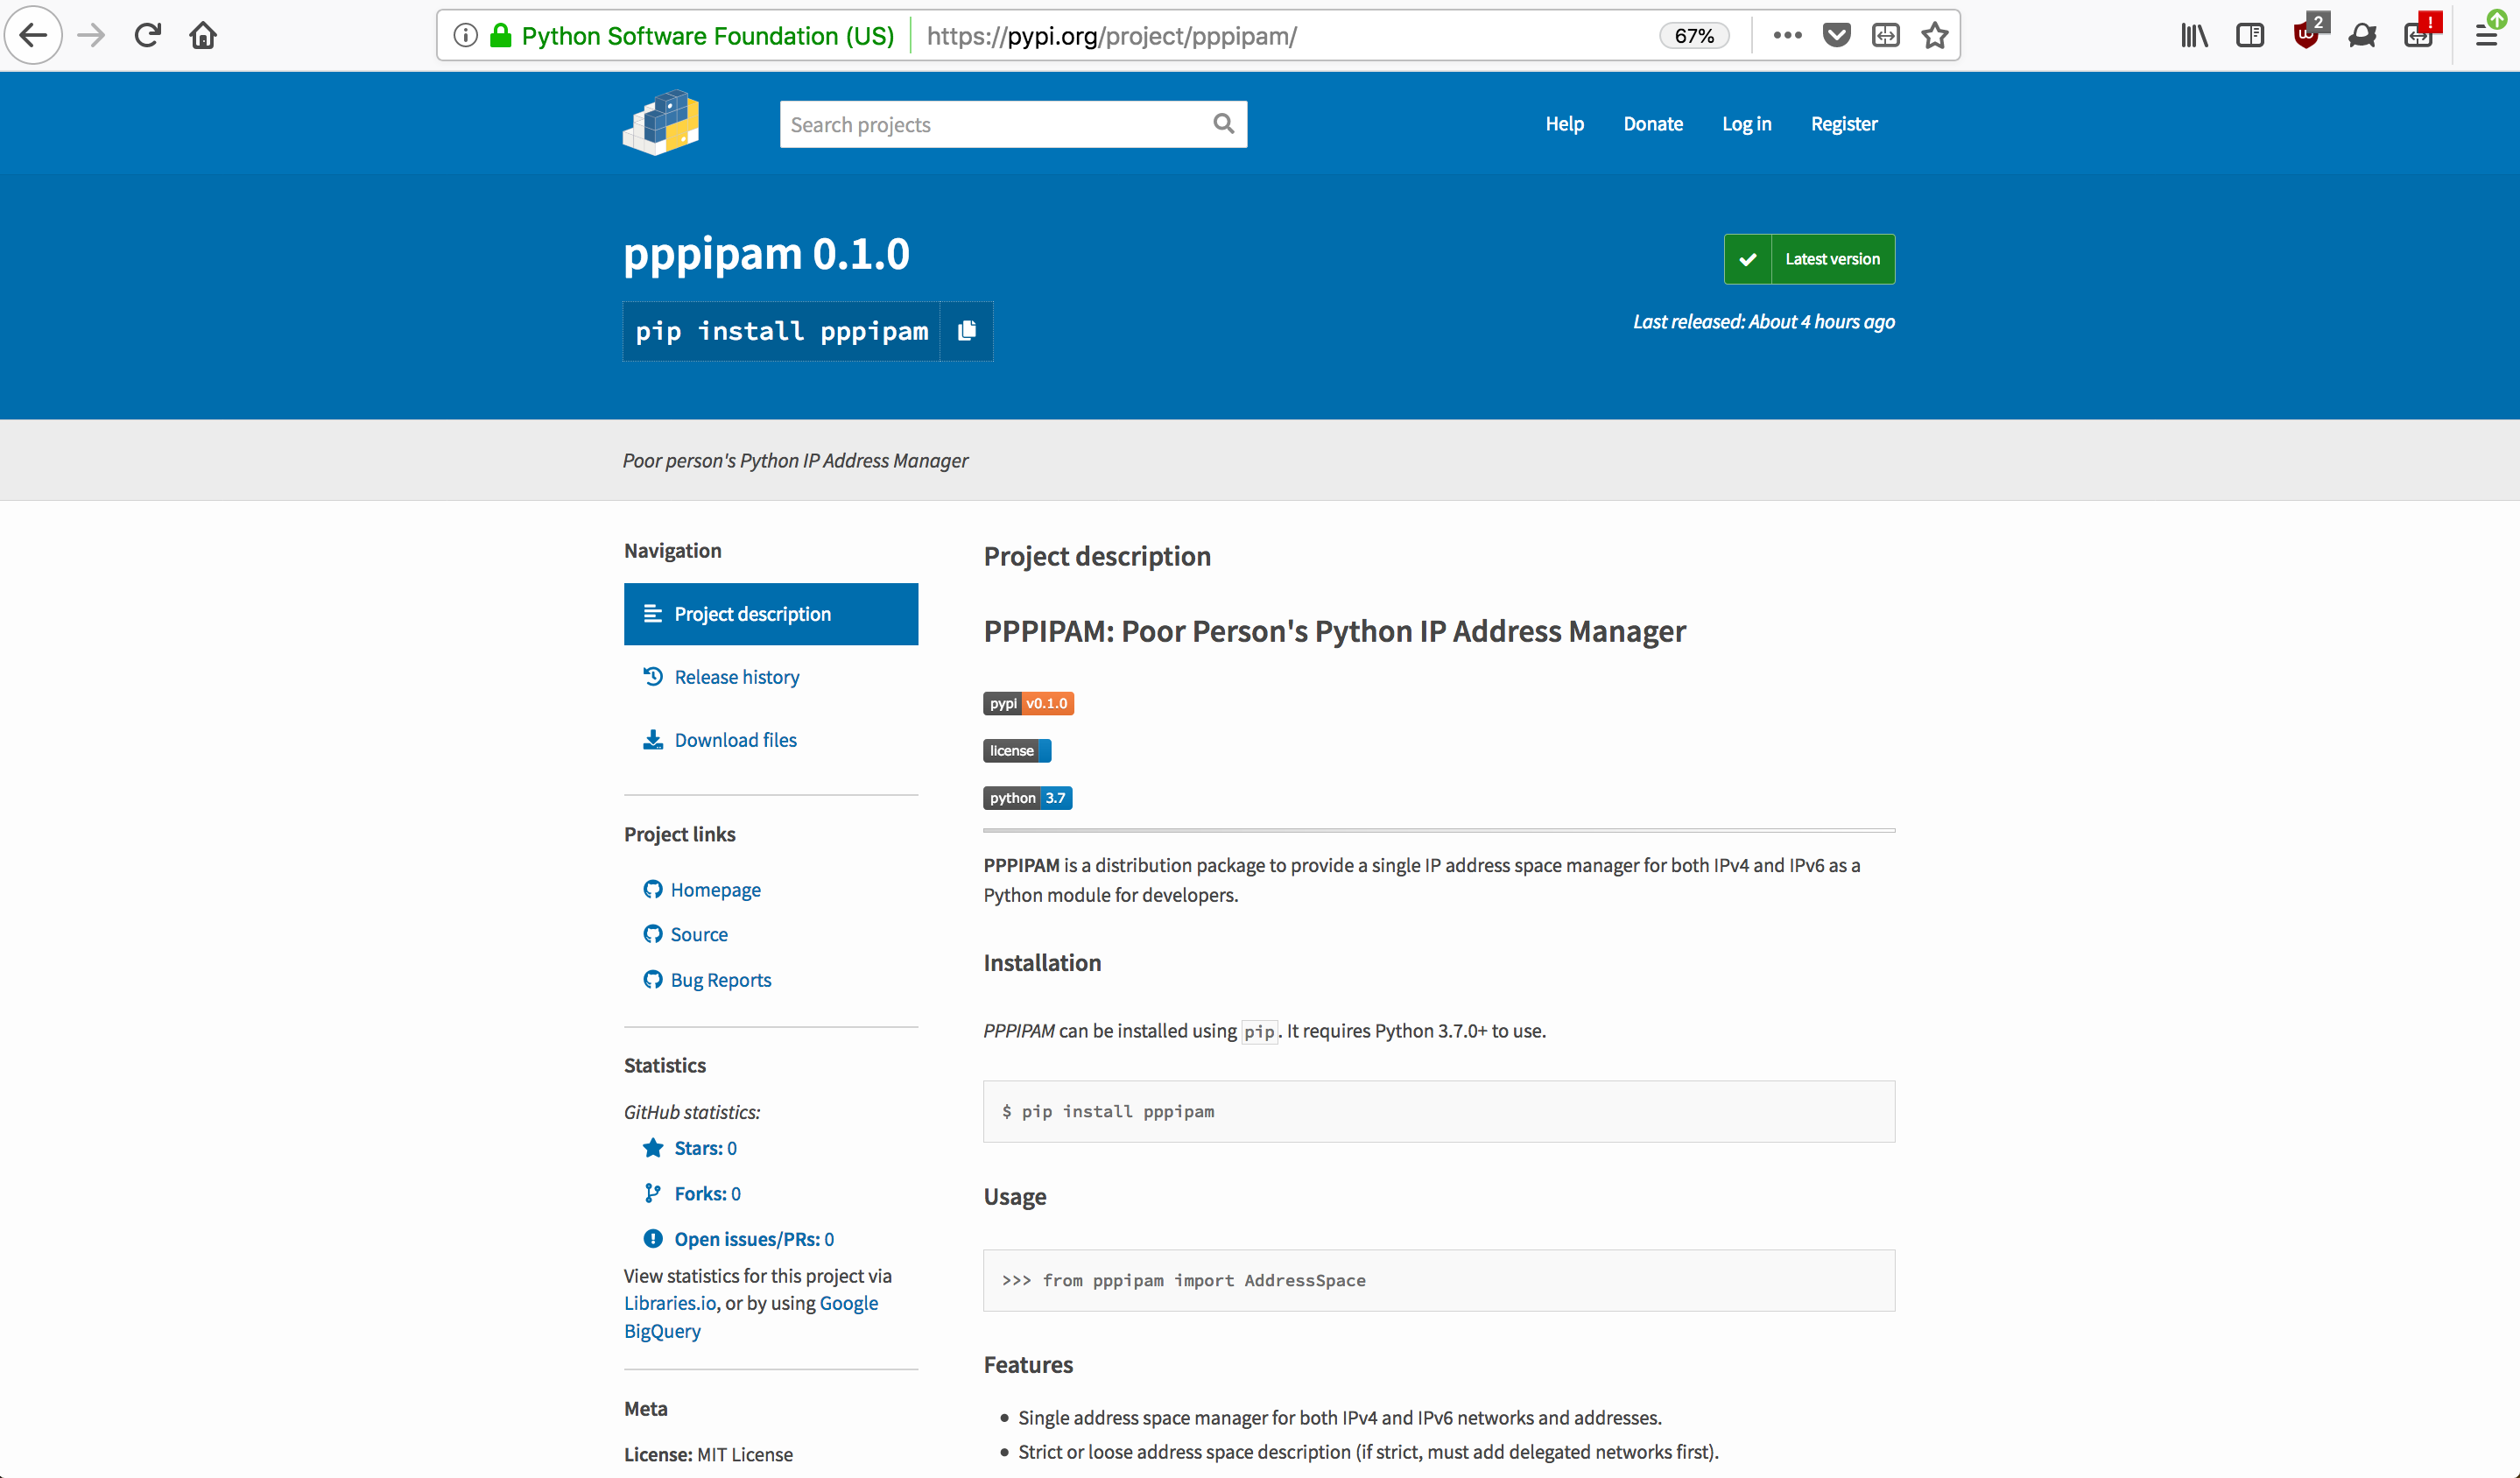
\includegraphics[width=12cm]{pypi_pppipam}}}
\end{frame}


\begin{frame}[fragile]
\begin{alltt}\footnotesize
\$ pip install pppipam
Collecting pppipam
  Downloading https://files.pythonhosted.org/packages/.../pppipam-0.1.0-py3-none-any.whl
Installing collected packages: pppipam
Successfully installed pppipam-0.1.0
\end{alltt}
\end{frame}


\begin{frame}[fragile]
\begin{alltt}\scriptsize
\$ python
Python 3.7.0 (default, Jun 29 2018, 23:55:57)
[Clang 9.1.0 (clang-902.0.39.2)] on darwin
Type "help", "copyright", "credits" or "license" for more information.
>>> from pppipam import AddressSpace
>>>
\end{alltt}
\end{frame}

\begin{frame}[standout]
\begin{alltt}
\$ pip3 install pppipam\newline
\newline
\$ python3\newline
>>> from pppipam import AddressSpace\\
>>>
\end{alltt}
\end{frame}


\begin{frame}[standout]
  \vspace*{2cm}
  \huge{Obrigado!}
  \begin{block}{}
    \vspace*{-.5cm}
    \begin{flushright}
      \large{\href{https://alexandre.harano.net.br/}{Alexandre Yukio Harano}} \\ \vspace*{0.1cm}
      \small{\href{mailto:alexandre@harano.net.br}{alexandre@harano.net.br}} \\
      \small{\url{https://alexandre.harano.net.br/}}
    \end{flushright}
    \vspace*{.2cm}
    \begin{flushleft}
      \normalsize{\url{https://github.com/ayharano/pppipam}}
      \normalsize{\url{https://pypi.org/project/pppipam/}}
      \normalsize{\url{https://github.com/ayharano/just-python/}}
    \end{flushleft}
  \end{block}
\end{frame}

\end{document}
